\documentclass[oneside,dutch]{tudelft-report}
\DeclareGraphicsExtensions{.pdf,.png,.jpg,.jpeg}
%\usepackage[numbered, framed]{mcode}
\usepackage{subcaption}
\usepackage{float}
\usepackage[dutch]{babel}
\usepackage{calc}  
\usepackage{enumitem}  
\usepackage{tabto}
\usepackage{adjustbox}
\usepackage{blindtext}
\usepackage{listings}
\usepackage{caption}
\usepackage{graphicx}
\usepackage{hyperref}
\usepackage{siunitx}



\title{\sffamily\Huge Final report}
\author{\sffamily\Large Projectgroep A5}
\affiliation{\sffamily TU Delft}
\date{\sffamily 14-01-2015}

\begin{document}
\maketitle

\chapter{Samenvatting}
Dit ontwerprapport is geschreven naar aanleiding van het project EPO-3 van het tweede jaar van de bacheloropleiding Electrical Engineering. In dit project staat het beschrijven van hardware centraal, met als doel het ontwerpen van een chip. In de keuze van een ontwerp zijn de studenten door de TU geheel vrij gelaten, er moest natuurlijk wel rekening worden gehouden met de grootte van de chip en het tijdsbestek waarin het ontwerp gerealiseerd kon worden. Er is hier door de EPO-3 groep A5 gekozen voor het ontwerpen van een spelcomputer, hierop kunnen meerdere spellen gespeeld worden. Om binnen het tijdsbestek te blijven is gekozen voor 'Pong', meerdere spellen kunnen eventueel achteraf simpel toegevoegd worden.

Van het uiteindelijke ontwerp wordt in de laatste periode van dit jaar een chip gemaakt, tijdens het ontwerpproces is er daarom met een FPGA development board gewerkt. Deze is geleverd door de TU Delft. Het grootste deel van het systeem bevindt zich op de chip zelf, toch zijn er nog drie losse componenten gebruikt om dit ontwerp te realiseren. Het idee achter de spelcomputer is dat hij meerdere spellen kan spelen, deze moeten extern aangeleverd worden. Er is hier gekozen voor een SD-kaart uitlezing met SPI, het spel is in assembly geschreven. Ook de besturing moest extern geregeld worden, met ultrasone sensoren bleek dit systeem het best te controleren. Als back-up plan is er hiernaast voor gekozen om ook enkele knoppen te implementeren. Om het spel te kunnen spelen is er tot slot ook een beeldscherm nodig.\\

Het belangrijkste deel van dit ontwerp bevindt zich op de chip. In de CPU wordt de informatie verwerkt die via SPI van de SD-kaart binnen komt. In de CPU wordt daarnaast ook de besturing van het spel verwerkt. De CPU kan dus gezien worden als het brein van de chip, alles wordt hier verwerkt en doorgegeven aan de GPU. Deze maakt er vervolgens een beeld van. Om vertraging op het scherm te voorkomen is er een 'Blackbox' geïmplementeerd, de zorgt ervoor dat er gewisseld kan worden tussen twee SRAM geheugens. Hierdoor kan er op de ene SRAM geschreven worden door de GPU en kan de ander worden uit gelezen door de VGA. De VGA produceert vervolgens het beeld op een beeldscherm. Alleen beide SRAM geheugen bevinden zich niet op de chip, maar ziten extern in het systeem verwerkt.\\

Tot in de laatste week is er hard gewerkt om alles op tijd werkend te krijgen, dit is helaas niet gelukt. Er is daarom besloten met de werkende onderdelen verder te gaan, van de ROM, CPU en de SPI decoder is een simpele rekenmachine ontworpen. De besturing loopt nog steeds via de sensoren in combinatie met enkele drukknoppen. De chip is nu in staat om enkele simpele berekeningen te doen, namelijk optellen, aftrekken en vermenigvuldigen.


\tableofcontents
\mainmatter

\chapter{Inleiding}
EPO-3 is het derde project uit de propedeuse van de bachelor opleiding Electrical Engineering aan de TU delft. Het doel van dit project is het ontwerpen van een chip, deze chip kan bijvoorbeeld een spelletje bevatten of als besturingsdoel dienen. Als project groep A5 is er gekozen voor het bouwen van een spelcomputer, hierop kunnen meerdere games gespeeld worden. De verschillende games moeten van een SD-kaart worden geladen voordat ze gespeeld kunnen worden. Het eerste spel dat ontworpen wordt is Pong, mocht er aan het eind van dit project nog tijd overblijven zullen er meerdere spellen volgen. De besturing loopt via ultrasone sensoren die de locatie van iemands hand bepalen. Het ontwerpen van een simpele spelcomputer sluit nauw aan met de bachelor opleiding Electrical Engineering. De toekomst van de elektrotechniek ligt dan ook in dit werkgebied. Chips zijn in de loop der jaren de basis gaan vormen voor bijna elk systeem. In dit ontwerprapport zal eerst het doel van dit project verder toe worden gelicht. Vervolgens zal er na het geven van het systeemoverzicht, wordt ieder individueel onderdeel beschreven. Testresultaten en codes zullen voornamelijk terug te vinden zijn in de appendices, tenzij anders aangegeven. 

\chapter{Probleemstelling}
\section{Projectopgave: 'Ontwerp een chip'}
De opdracht meegegeven door de TU is het ontwerpen van een chip. Hiermee is de gehele opdracht eigenlijk al beschreven, de studenten mogen verder in alle vrijheid de opdracht verder bepalen. Er wordt natuurlijk wel eerst grondig gecontroleerd door de tutoren of de opdrachten aan de eisen voldoen en haalbaar zijn.  Naast het ontwerpen van de chip mogen er extern onderdelen worden toegevoegd, bijvoorbeeld een beeldscherm of onderdelen voor de besturing. 

Als project groep A5 is er gekozen om van de chip een spelcomputer te maken, hierop moeten meerdere spellen gespeeld kunnen worden. Als eerst moet het spelletje 'Pong' te spelen zijn op deze spelcomputer. Aan het einde van het project kunnen eventueel andere spellen ontworpen worden. Extern moet er gezorgd worden voor besturing, weergave en opslag van de spellen. Dit laatste wordt door middel van een SD-kaart gerealiseerd. De besturing vind plaats via ultrasone sensoren of mocht dit niet naar behoren werken door middel van drukknoppen.

\section{Beschikbare infrastructuur}
In het 4e semester wordt de chip geproduceerd en getest, deze chip wordt door twee projectgroepen gebruikt. Elke groep heeft dus een halve chip voor zijn ontwerp, dit zijn ongeveer 200-250 flipflops. Daarnaast kan iedere groep wel gebruik maken van alle aansluitpinnen op de chip, dit zijn er 32. Voor het testen tussen door is er hardware beschikbaar, in de vorm van een Altera FPGA bord. Op dit Altera bord is veel randapparatuur aanwezig, daarnaast kunnen er nog andere externe onderdelen aan dit bord worden gekoppeld. 

\section{Functionele eisen}
Als functionele eisen kan er kortom gezegd worden dat er op de chip meerdere spellen gespeeld kunnen worden. Deze spellen moeten bestuurd kunnen worden door middel van ultrasone sensoren. Om te beginnen wordt 'Pong' ontworpen, andere spellen volgen als de projecttijd dit toelaat.

\section{Randvoorwaarden}
Aan het eindresultaat zitten een aantal randvoorwaarden verbonden. De externe onderdelen mogen maximaal 30 á 40 euro kosten, mochten deze niet voorhanden zijn. Er moet rekening worden gehouden met de grote van de chip. Tot slot dient aan alle tijdschema's te worden voldaan.

\section{Plan van aanpak}
Het plan van aanpak is een beschrijving van de aanpak van dit project, hierin staan onder andere de doelstellingen en wegen daar naar toe beschreven. Het plan van aanpak is te vinden in appendix A.

\chapter{Systeemoverzicht}
De spelcomputer ontworpen en gebouwd door EPO-3 groep A5 bestaat uit veel verschillende losse onderdelen. Om te voorkomen dat we het overzicht kwijt raken, wordt er in dit hoofdstuk het totale systeem beschreven. Er zal dus vooral worden gekeken naar de toplevel beschrijving, hierin worden alle onderdelen samengevoegd en gekoppeld tot een geheel. Ook wordt er in het kort even ingegaan op de externe componenten die ons systeem bevat.

\begin{figure}[H]
\center
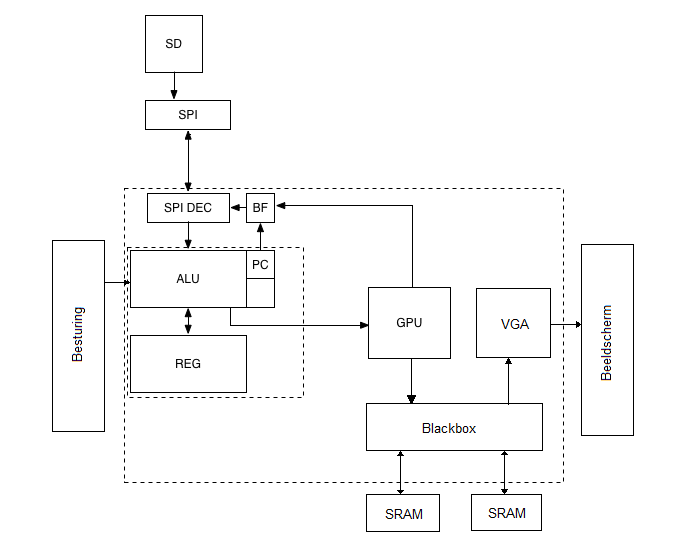
\includegraphics[width=9cm]{hele-systeem}
\caption{Totale systeem weergave}
\label{Systeemoverzicht}
\end{figure}

\section{Toplevel}
De toplevel beschrijving bestaat uit een entity en een behaviour. In de code van de entity staan alle poorten beschreven die de chip verbinden met de externe componenten die het systeem bevat. In de behaviour worden alle interne componenten aan elkaar verbonden. In figuur \ref{Systeemoverzicht} staat schematisch weergegeven op welke manier dit gebeurd. De losse onderdelen van dit systeem worden individueel beschreven in dit verslag.

\section{Externe componenten}
Het systeem dat ontworpen is door EPO-3 groep A5 bevat kort gezegd drie aparte externe componenten, twee daarvan zijn inputs en een is een output. De inputs van dit systeem zijn de besturing en de opslag van het spel. Dit laatste gebeurd door middel van SD uitlezing met SPI. De output van dit systeem wordt aangestuurd door de VGA en kan een beeld produceren op een willekeurig beeldscherm.

\chapter{Besturing}
Ons systeem wordt gespeeld doormiddel van 2 soorten besturing. De Ultrasone en de Button. De speler kan de modus selecteren doormiddel van een switch. Deze data van de buttons en de ultrasone worden verwerkt door een Arduino. Er is gekozen voor deze optie omdat de Arduino via SPI werkt. Hierdoor kan de SPI code getest worden en kunnen we het aantal pinnen dat gebruikt wordt laag houden. 

\section{Ultrasone}
Een unieke uitdaging van ons project is de Ultrasone besturing, de besturing werkt door middel van een (ultrasone)sensor aan de rechterzijde van de speler. Deze sensor meet met een speel ruimte van 75cm elke 11 milliseconde. Het aansturen van de ultrasone sensoren gaat doormiddel van een 2ms lange pulse op de IN-pin. Dit is de trigger van de SRF-04(de door ons gekozen ultrasone sensor). Hierna verzend de sensor zijn pulse, op dat moment wordt de OUT-pin ook hoog. Deze blijft hoog tot de gereflecteerde pulse weer binnen komt. Deze tijd wordt gedeeld door 2 omdat het geluid zowel de afstand heen als terug moet afleggen. Deze tijd wordt vervolgens geschaald naar afstand door hem door 29m/s(de snelheid van geluid in lucht) te delen. Hierna wordt de tijd teruggemapt(alles tussen de 0 en de 75 wordt terug geschaald naar 0 en 12). Deze waarde wordt voor player 2 4 bits geschoven naar links. En vervolgens wordt het signaal via de hierbovengenoemende SPI verstuurd naar de chip.

\section{Buttons}
Bij de buttons wordt een andere manier van werken gehanteerd, hier wordt de waarde van de plaatsvector onthouden(als integer). En naar gelang welke button geactiveerd wordt, wordt het signaal 1 verhoogd/verlaagd. Dit getal kan maximaal 12 bereiken en minimaal 0. Vervolgens wordt dit signaal voor player 2 ook verschoven, en daarna verzonden via SPI.

De getallen 0->12 voor player 1/2 zijn in gebruik, dit geeft ruimte om 13,14,15 te gebruiken voor andere doeleinde. 13 dient als getal om de Start van systeem aan te geven. 15 is de Reset van het systeem.

\section{SPI-communicatie}
Alle variable die berekent worden in de arduino worden via SPI verzonden. SPI is een protocol over het verzenden van de data. Dit werkt doormiddel van 2 draden. Draad 1 verzend een klok van 8 pulse lang en een default low. Draad 2 verzend de waarde van 8 bits lang.

\section{Detectie SPI}
De chip detecteerd op de opgaande flank van draad 1(klok) de waarde van draad 2(signaal). Deze waarde wordt in een Flip-flop(geheugen) gezet. Op de neergaande flank wordt de waarde geshift. Dit moet om te zorden dat de data in de goede volgorde aankomt bij de CPU.

\section{Simulatie}
Na de ontwikkeling via Go-with-the-flow is het systeem getest. Hierbij is gebruik gemaakt van een dubbele 6 als positie. Het resultaat ziet u in: 
\begin{figure}[H]
\center
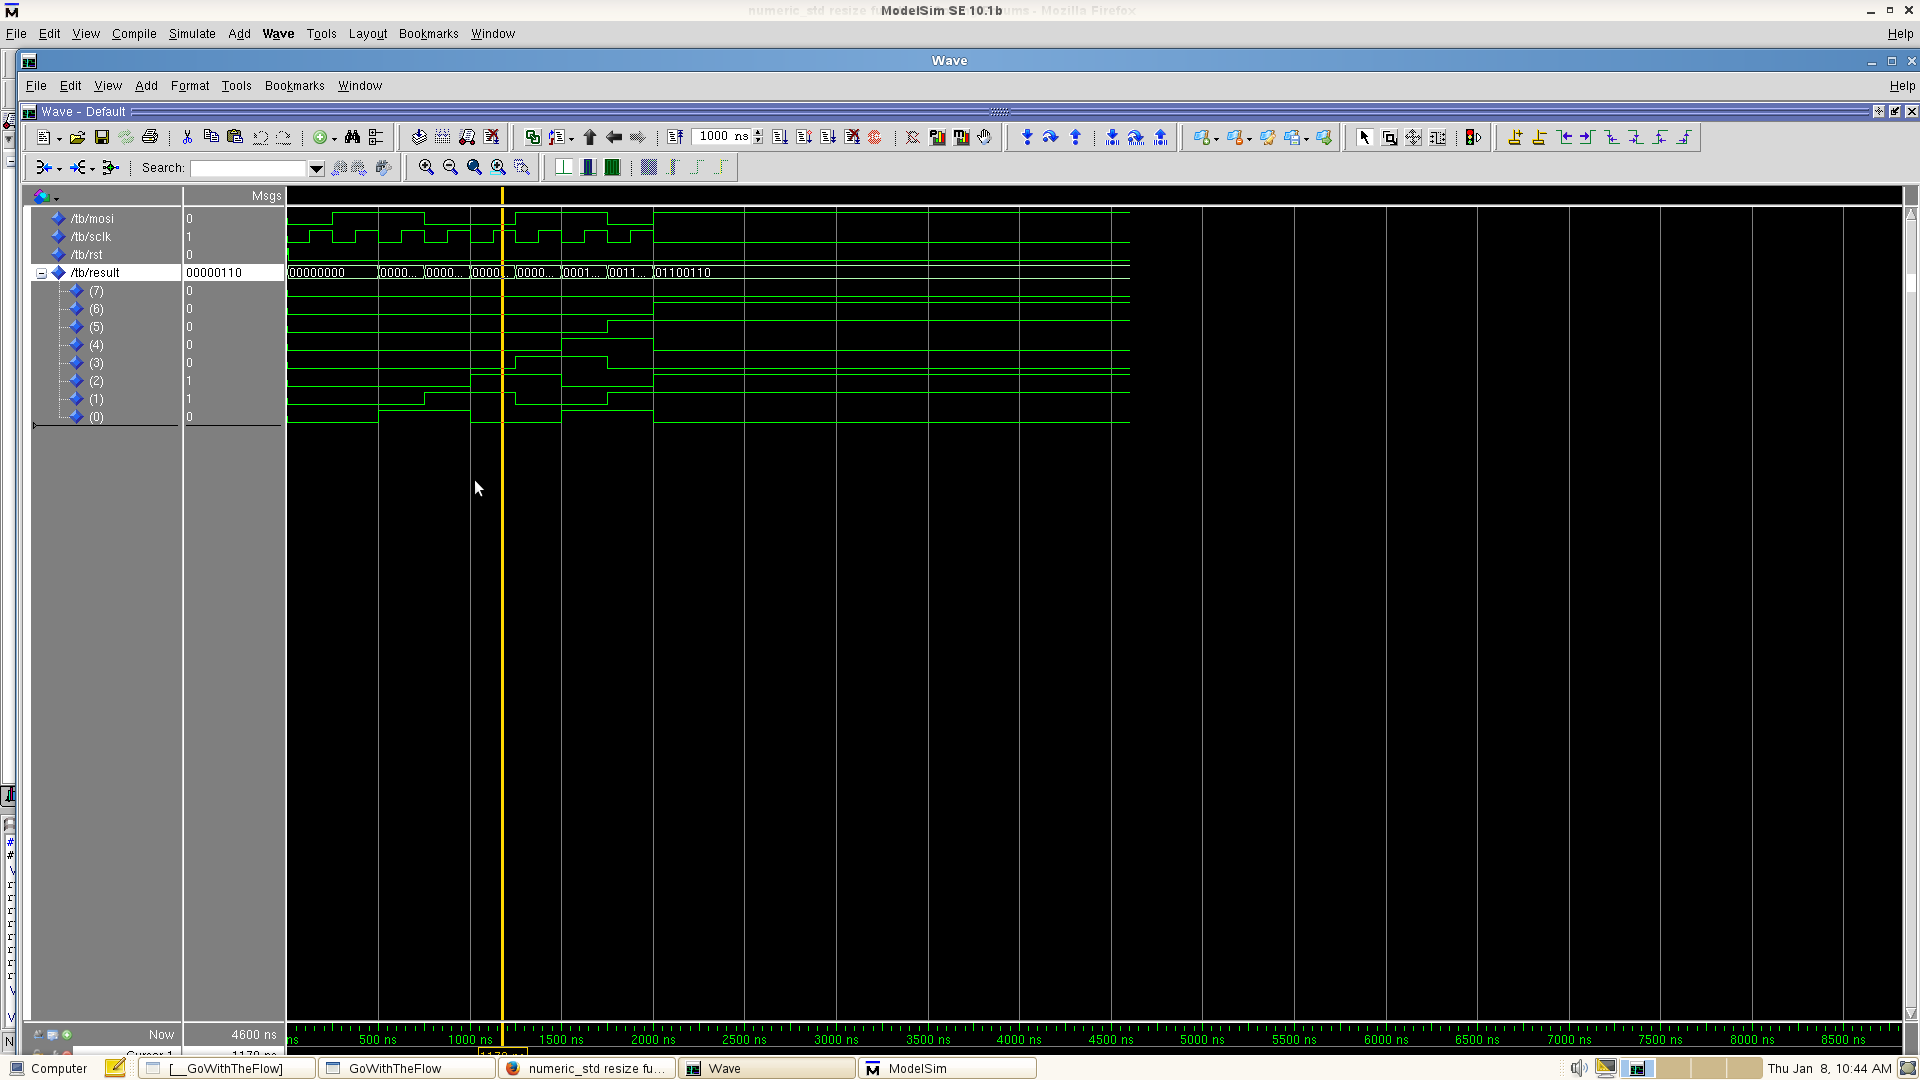
\includegraphics[width=9cm]{Screenshot.png}
\caption{Twee maal de positie 6 gemeten met Modelsim}
\label{CPU}
\end{figure}

Vervolgens is het systeem gedownload op de FPGA, hierop is de arduino aangesloten. Het signaal van de arduino was:
\begin{figure}[H]
\center
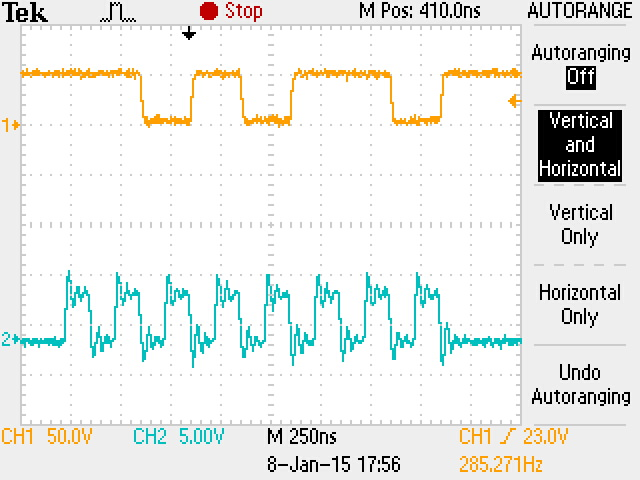
\includegraphics[width=9cm]{TEK0001.JPG}
\caption{De positie 13(start) en 6}
\label{CPU}
\end{figure}
Deze waarde kwam precies zoals verwacht op de ledjes op de FPGA. Echter na ongeveer 5 seconde begon de waarde te shiften. Dit kwam door dat beide systemen geen gecombineerde aarde had. Dit is opgelost door een draad tussen beide aarde te zetten.


\newpage


\chapter{Blackbox}
\section{Functionele beschrijving}
Voor het genereren van de beelden worden twee SRAM chips gebruikt. De ene chip wordt uitgelezen door de VGA generator en er wordt naar de andere chip geschreven door de GPU. Als een frame geschreven is naar de SRAM chip wordt de chip waar net naar geschreven is verbonden met de VGA generator zodat deze uitgelezen kan worden. De chip die voorheen verbonden was met de VGA wordt doorverbonden met de GPU zodat daar vervolgens naar geschreven kan worden. Door deze techniek toe te passen blijft het beeld op het scherm stabiel. De BlackBox is de schakeling die dat mogelijk maakt.
\section{Inputs en outputs}
De SRAM chips, de VGA en de GPU communiceren met elkaar met behulp van SPI. De schakeling heeft dus twee SPI master aansluitingen voor VGA en de GPU en twee SPI slave aansluitingen voor de twee SRAM chips. Een SPI aansluiting bestaat uit vier signaallijnen. Dit zijn de serial clock (SCLK), master in slave out (MISO), master out slave in (MOSI) en slave select (SS). Ook heeft de schakeling nog een ingang om te selecteren welke SRAM chip verbonden is met de VGA generator en welke met de GPU.

\begin{figure}[H]
\center
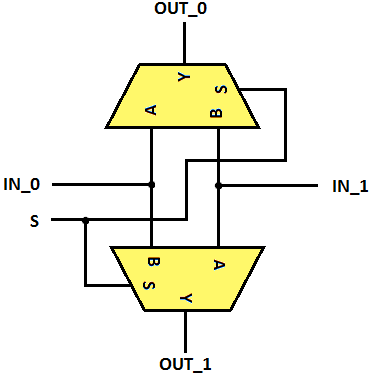
\includegraphics[width=9cm]{./BlackBox_Circuit}
\caption{Subschakeling van de blackbox}
\label{sub-blackbox}
\end{figure}

\section{Implementatie}
De schakeling bestaat uit vier subschakelingen. De subschakeling bestaat uit twee twee naar 1 lijn multiplexers zoals weergegeven in figuur \ref{sub-blackbox}. Door de S laag te maken, wordt IN\_0 verbonden met OUT\_0 en IN\_1 met OUT\_1. Als S hoog is, is IN\_0 verbonden met OUT\_1 en vice versa. Vervolgens worden de SCLK lijnen van de GPU en VGA generator verbonden met de ingangen van de subschakeling en de uitgangen met de SCLK lijnen van de twee SRAM chips. Hetzelfde gebeurt ook voor de MOSI en de SS lijnen van de masters en de slaves. Bij de MISO lijnen is het omgekeerd omdat dit een inputlijn is voor de masters en een outputlijn voor de slaves. Hier worden dus de SRAM chips verbonden met de ingangen en de VGA generator en de GPU aan de uitgangen. De BlackBox bestaat nu uit vier subcircuits. Door de select (S) ingangen van de subschakelingen met elkaar te verbinden is de BlackBox nu compleet.
\section{Simulatie}
Om de werking van de schakeling te verifiëren is een switch-level simulatie gedaan zoals te zien is in figuur \ref{bbsls}. 

\begin{figure}[H]
\center
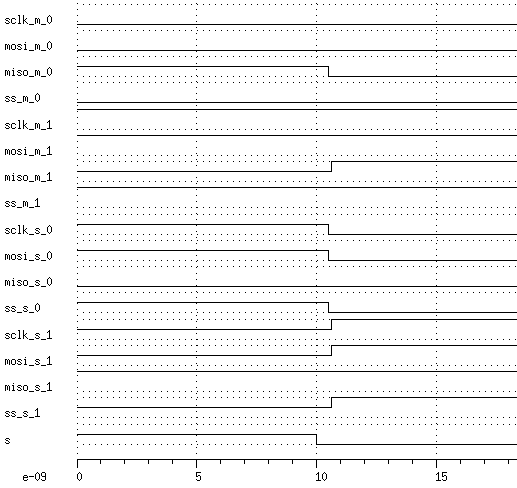
\includegraphics[width=9cm]{./BlackBox_SLS}
\caption{Switch-Level Simulation van de blackbox}
\label{bbsls}
\end{figure}

Er valt te zien dat voordat het signaal s hoog wordt de SPI signalen van master 0 en slave 0 overeenkomen. Ook de spi signalen van master 1 en slave 1 komen overeen. Nadat s laag wordt zien we dat de signalen van master 0 nu overeenkomen met de signalen van slave 1 en vice versa. Hieruit kan geconcludeerd worden dat de schakeling naar behoren zou moeten werken wanneer deze geïmplementeerd is in de chip. De schakeling kan getest worden door de signalen op de bijbehorende pinnen te bekijken en deze te vergelijken met de verwachte signalen van de SPI van de GPU en VGA circuits. 

\newpage

\chapter{CPU}
\section{Functionele beschrijving}
Om programma’s uit te kunnen voeren wordt gebruik gemaakt van een door de Delta-1 [INSERT BRON HIER] geïnspireerde microprocessor. Deze 8-bits processor krijgt instructies binnen die via SPI van een SD-kaart worden afgelezen. Vervolgens voert de processor bewerkingen uit, waarvan de resultaten doorgestuurd worden naar de overige componenten op de chip. De data die uit de processor komt wordt hierna door de VGA-controller omgezet naar beelden op het scherm.



\section{Inputs en outputs}
De processor heeft in totaal vijf ingangen. Dit zijn de 12-bits instructie-bus waarop de instructies staan die vanaf de SD kaart worden afgelezen, een 8-bits signaal waar alle externe inputs op komen te staan, de reset en het CPU-enable signaal. Het CPU-enable signaal geeft door aan de processor dat een nieuwe instructie klaar staat om uitgevoerd te worden. Op het 8-bits signaal waar alle inputsinformatie op staat, staat bijvoorbeeld welke knoppen ingedrukt zijn bij de besturing.
We hebben besloten om de CPU niet te laten draaien op een kloksignaal, maar op het enable signaal. Op deze manier voert de CPU iedere keer dat er een instructie op de ingang wordt aangeboden één enkele instructie uit. Zo gaat de CPU geen ongewenste stappen ondernemen met verkeerde/verouderde ingangswaardes. 

Verder beschikt de CPU over twee uitgangen: Eén 8-bits signaal dat data naar de VGA controller stuurt en een 8-bits signaal dat het adres van de volgende instructie doorgeeft aan de SD-kaart uitlezer. 

\begin{figure}[H]
\center
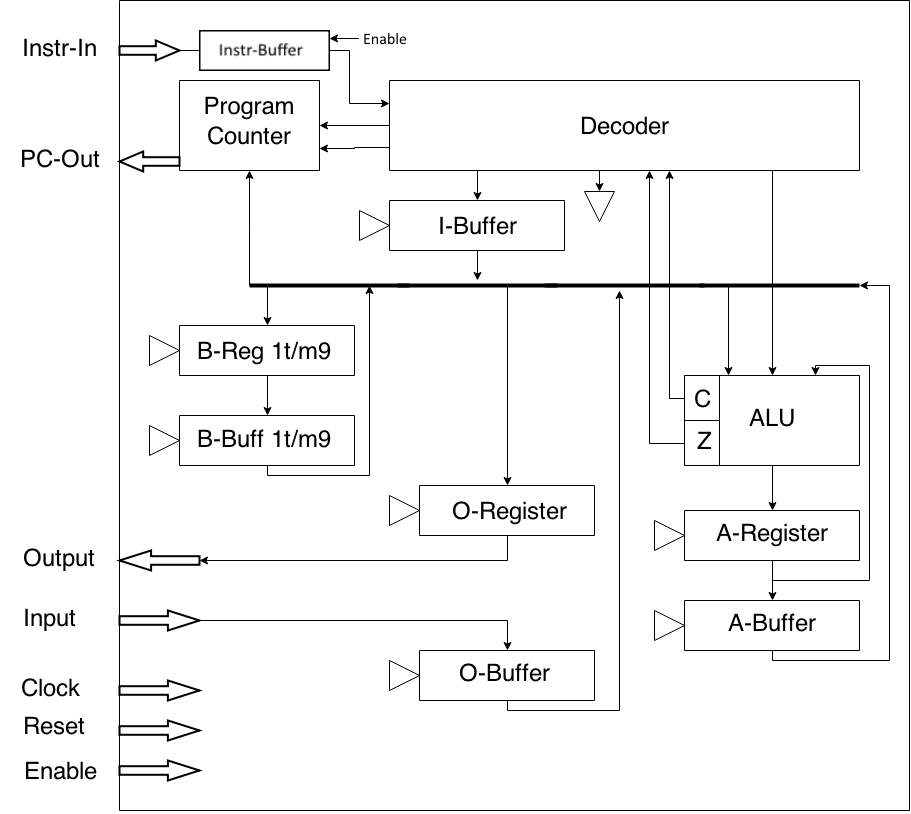
\includegraphics[width=9cm]{CPU-toplevel2}
\caption{Toplevel beschrijving}
\label{CPU}
\end{figure}


\section{Implementatie}
De totale processor is opgebouwd uit vijf verschillende sub-schakelingen: Registers, buffers, een rekenkern, een program-counter en een instructie-decoder.

De processor beschikt in totaal over elf registers. Wanneer het enable-signaal vanaf de decoder van een register hoog is, slaat deze de waarde die op dat moment aan zijn ingang staat op en kan deze data bij een latere bewerking weer uitgelezen worden. Hiervan worden er negen gebruikt om waarden op te slaan voor volgende bewerkingen, één om data aan de data-uitgang van de processor te zetten en één aan de uitgang van de rekenkern om direct een volgende bewerking op uit te kunnen voeren. Het enable-signaal staat in een 5-bits vector, waarmee ook de registers waarin je data wilt opslaan geselecteerd worden. De most-significant bit bepaald of de register enabled is. De overige vier bits is het adres van het register dat je wilt selecteren.

Verder zijn er dertien buffers aanwezig. Deze buffers laten data van hun ingang door naar hun uitgang wanneer hun enable-signaal vanaf de decoder hoog is, en geven 'high-Z' aan de output door wanneer dit niet zo is. Ze maken dus data beschikbaar aan de bus, zodat er verder mee gerekend kan worden. Negen van deze 8-bits buffers staan tussen de uitgangen van de opslag-registers en de databus, één aan de controller-input, één tussen het rekenkern-register en de databus, één die vanuit de decoder een numerieke waarde op de databus kan zetten en één 12-bits buffer aan de instructie-ingang van de CPU. De negen buffers achter de opslag-registers worden op dezelfde manier geselecteerd als de registers, maar dan op hun eigen data-bus.

De Arithmetic Logic Unit (ALU) heeft één 3-bits instructie-ingang vanuit de decoder, twee 8-bits data ingangen waarvan er een van de databus komt en een het resultaat van de vorige bewerking bevat, een 1-bit carry uitgang die aangeeft wanneer er een overflow optreedt bij een optel-operatie, een 1-bit zero uitgang die aangeeft wanneer een 'AND' operatie enkel nullen oplevert en een 8-bits uitgang waar het resultaat van de bewerkingen op staat. Afhankelijk van het instructie-signaal wordt een andere operatie uitgevoerd met de data op de twee ingangen.
Op basis van de Opcode selecteert de ALU middels 'when' statements welke functie hij moet uitvoeren.

De Program counter krijgt na elke instructie van de decoder een signaal om ofwel één instructie verder te gaan, of om naar een specifieke instructie te 'springen'. Dit wordt gedaan met behulp van een 1-bit increment en -jump signaal. Zolang de increment ingang hoog is wordt er telkens één opgeteld bij iedere instructie, en als het jump signaal hoog is wordt het nieuwe instructie-nummer vanaf de databus uitgelezen. Het 8-bits uitgangssignaal bevat het adres van de volgende instructie en wordt doorgegeven naar de SD-kaart uitlezer. De program counter zal bij elk opgaand enable signaal een stap verder gaan, dus bij iedere nieuwe instructie wordt gekeken wat de volgende instructie gaat zijn.


Aan het hoofd van de processor bevindt zich de instructie decoder. Deze decoder stuurt naar aanleiding van een 12-bits instructie de overige componenten binnen de CPU aan. Dit wordt gedaan door eerst het 12-bits signaal op te delen in een 4-bits instructie en een 8-bits argument. Hierna wordt afhankelijk van de instructie een enable-signaal naar een relevant register of buffer, een instructie-code naar de rekenkern en een increment of jump signaal naar de program counter gestuurd. Het 8-bits argument kan ofwel als waarde op de databus gezet worden of als enable-signaal omgezet worden voor een register of buffer. De mogelijke instructies met bijbehorende uitgangssignalen van de decoder zijn te zien in tabel [figuur \ref{Instructie}]. In de tabel is te zien bij welke ingangssignalen de output hoog moet zijn. Met dit in gedachten kan door middel van logische combinatoriek voor iedere uitgang een logische functie worden gedefinieerd.

De volledige layout is te zien in \autoref{CPU}, en de mogelijke instructies met bijhorende interne signalen zijn te zien in \autoref{Instructies}

\begin{figure}[H]
\begin{center}
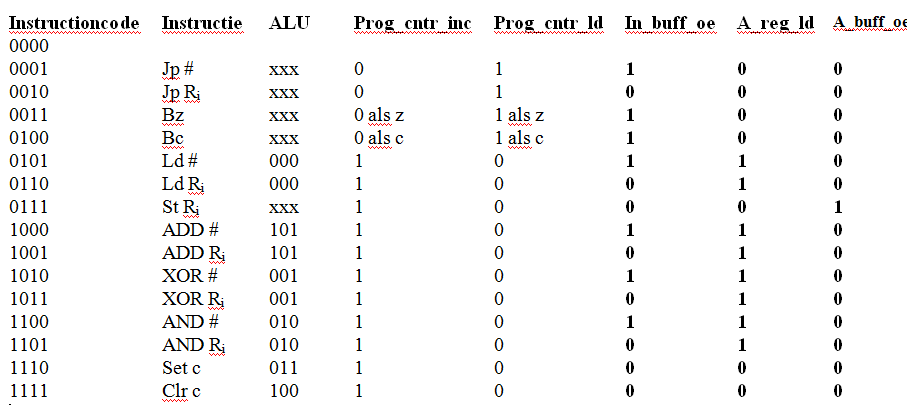
\includegraphics[width=12cm]{tabel}
\caption{Instructies met bijbehorende uitgangssignalen}
\label{Instructies}
\end{center}
\end{figure}


\chapter{GPU}
\section{Doelstelling}
De GPU dient als vertaalslag tussen de 8-bit commando’s welke worden ontvangen vanuit de output buffer van de CPU, en de pixelmap welke opgeslagen is in het SRAM. Door het gebruik van 2 wisselende SRAM chips kan de GPU in de ene SRAM chip schrijven, terwijl de VGA-module uit de andere SRAM chip aan het lezen is. De GPU ontvangt vanuit de CPU achtereenvolgens commando’s met hierin data van de X en Y posities van de in te kleuren pixel. Tevens is er een commando aanwezig om het volledige scherm leeg te vegen.

\section{I/O}
De I/O van de GPU zal bestaan uit de communicatie met de CPU, SPI uitgang naar het SRAM en klok- en resetsignalen ten behoeve van het realiseren van de FSM’s.



\subsection{Input CPU}
De ingang van de CPU zal bestaan achtereenvolgens 8 bit commando’s welke zullen worden opgesplitst in een 2 bit commando, en een 6 bit datavector. Zie onderstaande tabel.\\


\begin{tabular}{| c | c | c | c | c | c | c | c | }
 \hline			
  7 & 6 & 5 & 4 & 3 & 2 & 1 & 0  \\ \hline
instruction(1) & instruction(0) & data(5) & data(4) & data(3) & data(2) & data(1) & data(0) \\
  \hline  
\end{tabular} \\
\\

De instruciteset van de GPU worst als volgt gedefinieerd:
\begin{description}
\item ["01"]
	Read X: Deze instructie beschrijft dat de CPU in de databits de x-coördinaat van de in te kleuren pixel weergeeft. 
\item ["10"]
	Read Y: Deze instructie beschtijft dat de CPU in de databits de y-coordinaat weergeeft van de in te kleuren pixel.
\item ["11"]
	Clear screen: Deze instructie geeft aan dat de volledige pixelmap in het SRAM leeggemaakt kan worden.
\end{description}


\subsection{SPI}
De uitgang van de GPU zal bestaan uit SPI signalen om te comminuceren met het SRAM. Gedurende het project is gebleken dat het noodzakelijk blijkt te zijn dat de GPU zowel kan lezen als schrijven vanuit het SRAM. Dit betekend dat er een volledig bidirectionele comminucatie vereist is tussen SRAM en GPU. De comminucatie met het gekozen SRAM zal worden gerealiseerd volgens de door de datasheet van het SRAM opgegeven commando's. Voor de GPU zijn de lees en schrijf commando's van belang. Deze zijn te vinden in figuur \ref{sram}.


\begin{figure}[H]
\center
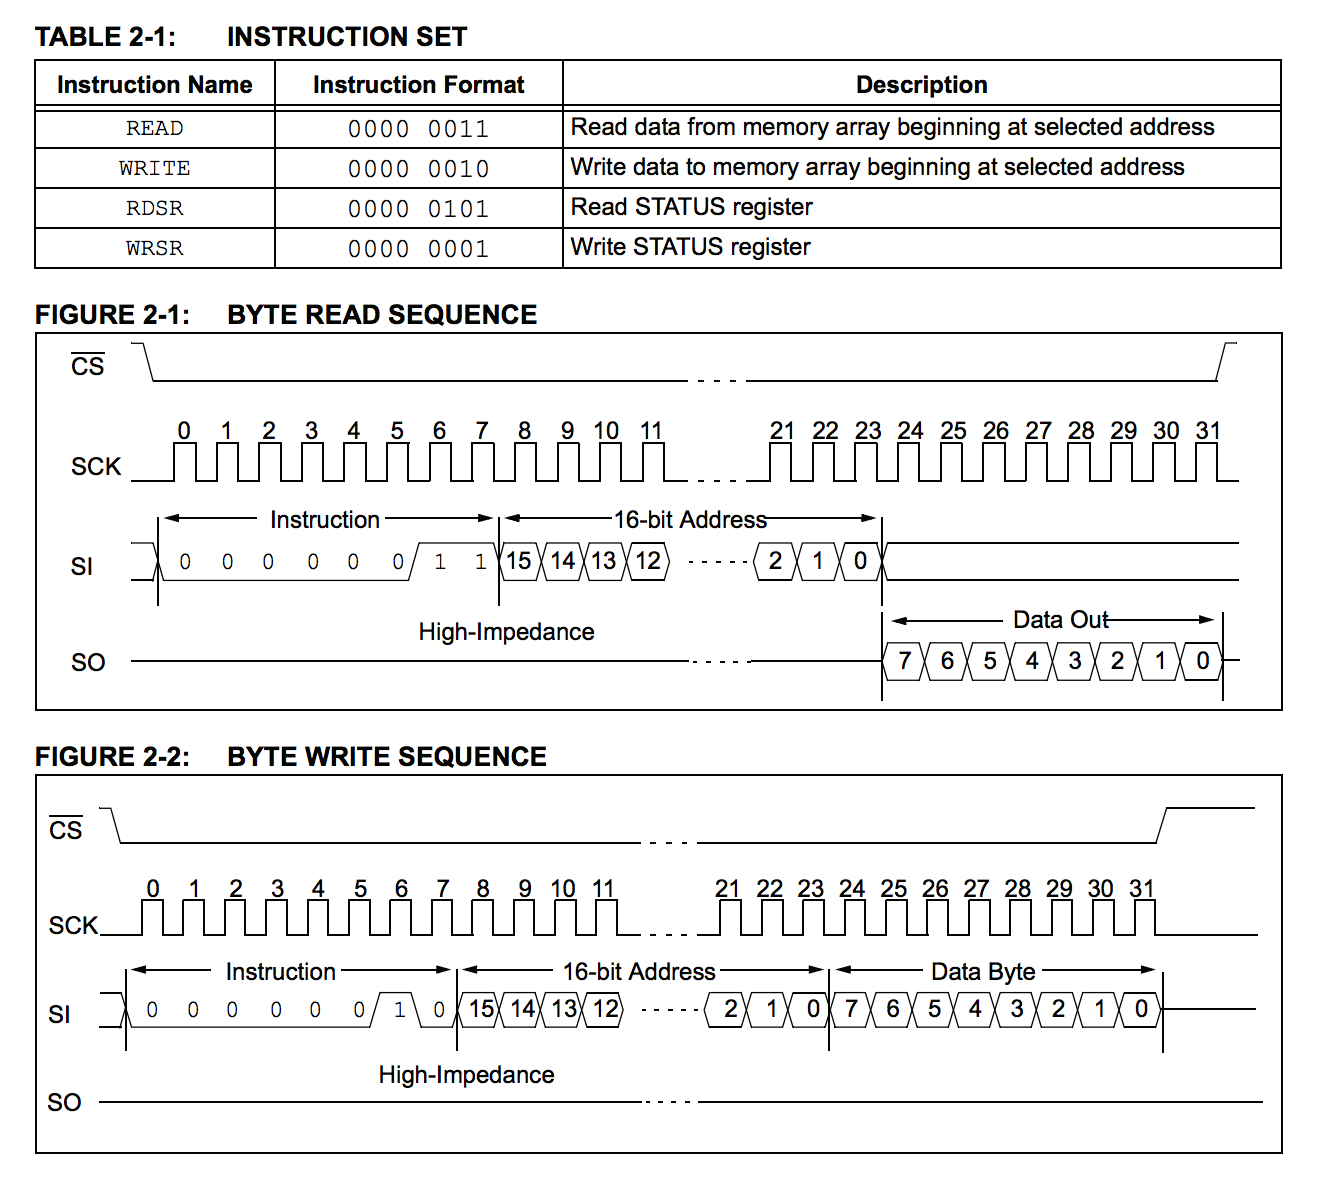
\includegraphics[width=15cm]{sramcomm}
\caption{SPI specificatie volgens datasheet SRAM}
\label{sram}
\end{figure}

\section{Randvoorwaarden}
Tijdens het ontwerpen van de FSM ten behoeve van de GPU zal het noodzakelijk zijn om deze te laten voldoen aan een aantal gestelde randvoorwaarden met betrekking tot de comminucatie met andere compnoneten.
\subsection{Indeling beeldscherm}
De indeling van het uiteindelijke beeldscherm wordt deels bepaald door de GPU, gedurende het ontwerpprocess is er uit gegaan van de volgende beeldschermspecificaties.
\begin{description}
\item[Pixeldefinitie]
	De resolutie van het scherm is vastgesteld op 32 bij 24 pixels. Dit betekend dat de maximale ingangswaarde van de databits van de CPU 32 zal zijn, en dit getal prima in de 6 bit vector past.

\item[Kleuren]
	Er is tijdens het ontwerp besloten om geen gebruik te maken van kleuren, dus enkel zwart en witte pixels.

\item[Bits in Bytes]
	De pixelmap van het beelscherm zal in het geheugen worden als bytes, waarin elke bit een ingekleurde pixel voorsteld. Bij de logische waarde '1' zal de pixel ingekleurd worden. Zie figuur \ref{pixelmap} voor een grafische representatie van de pixelmap in bytes, en figuur \ref{bit} een representatie van de indeling van 1 individuele byte. In de pixelmap is te zien dat er exact 1 byte buiten het scherm valt in verband met de back proch van het beeldscherm.
\end{description}

\begin{figure}[H]
\center
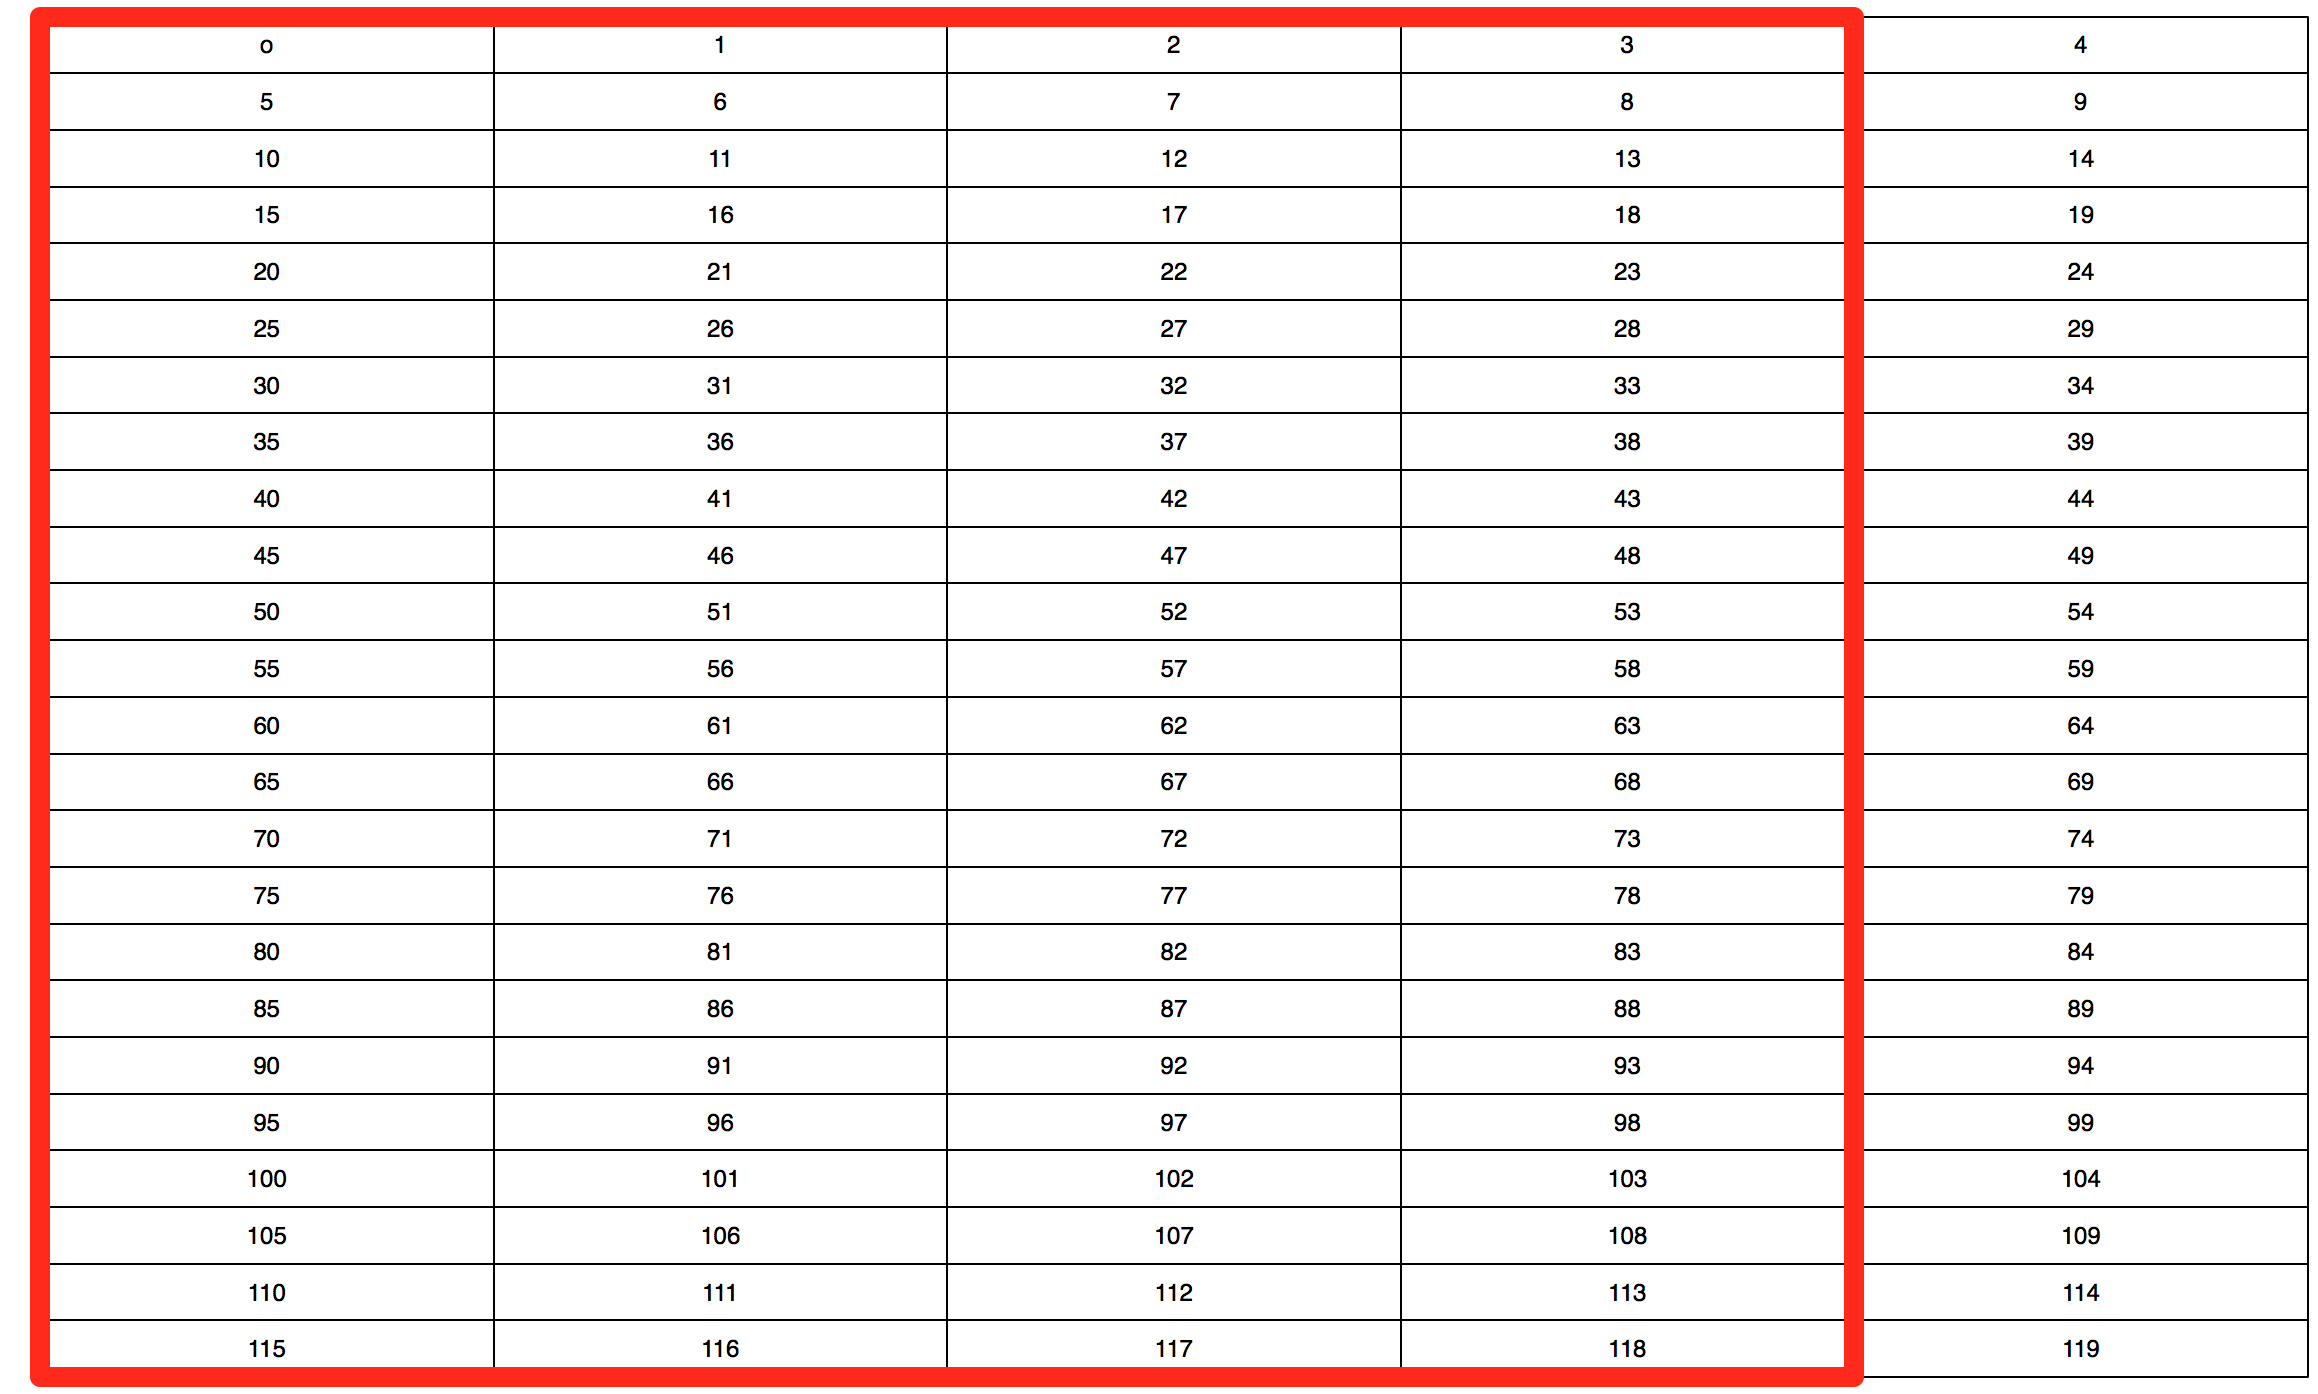
\includegraphics[width=15cm]{pixelmap}
\caption{Pixelmap, rood kader is beelscherm}
\label{pixelmap}
\end{figure}

\begin{figure}[H]
\center
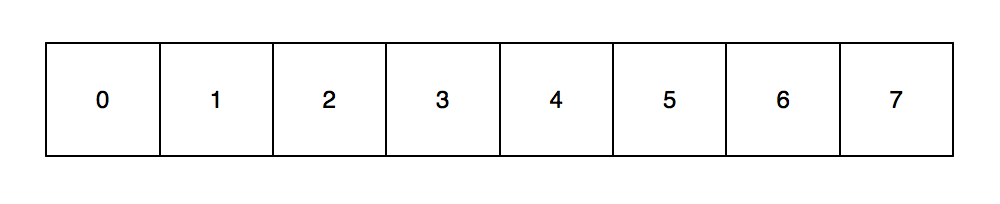
\includegraphics[width=9cm]{byte}
\caption{Indeling byte}
\label{byte}
\end{figure}


\section{Processes}
De CHDL code van de GPU bestaat uit een drietal processes welke voor de verwerking van de gegevens zorgen.
\subsection{Process 1 : State-Renew}
Het state renew process heeft als taak om bij elke opgaande klokflank de nieuwe state toe te wijzen aan het register waar de huidige state in is opgeslagen. Tevens heeft dit proces als doel om te reageren op een actief reset signaal, waarin er voor de nieuwe state een specefieke resetstate wordt toegewezen (State[0]).
\subsection{Process 2 : Counter}
De counter wordt gerealiseerd door een 11 bits unsigned waarde welke gebruikt kan worden binnen de FSM om bijvoorbeel het aantal onvangen bits via SPI te tellen. De teller reageeert net zoals voorgaan process op de opgaande klokflank.
\subsection{Process 3 : FSM}
De FSM van de GPU doet de daadwerkelijke berekeningen en vertaalslagen. In figuur \ref{fsmgpu} is een overzicht te vinden van de volledige FSM. Onderstaand zullen de verschillende functieblokken besproken worden.
\begin{description}
\item [Blok A]
	Blok A is de resetstate van de volledige FSM. In blok A is de FSM gevoelig voor veranderingen op de instructieingang van de CPU. Zo kan de FSM overgaan naar state[13] wanneer het commando voor 'clear screen' gegeven wordt, of naar stat[1] wanneer deze een x-coordinaat ontvangt. Voor het tijdelijk opslaan van x en y waarden van de CPU wordt gebruik gemaakt van 2 8-bit buffers, welke gedurende state[0] worden gereset om te garanderen dat de volgende berekening geen oude resultaten meedraagt.
\item [Blok B]
In blok B wordt het y-coordinaat ontvangen en zal de FSM berekenen in welke byte in het geheugen de pixel weggeschreven zal worden. Tevens wordt hier de instructie klaargemaakt om data vanuit het SRAM te lezen.
\item [Blok C] 
	Blok C zal met behulp van de counter het sclk signaal genereren, en de lees instructie, met daarin tevens het adres van de te lezen byte verzenden naar het SRAM.
\item [Blok D]
	Blok D zal de 8-bit byte van het SRAM ontvangen en deze opslaan in een daarvoor bestemde buffer.
\item [Blok E]
	Blok E berekend op welke plaats in de byte een '1' geschreven zal moeten worden en vergelijkt dit met wat er reeds in de ontvangen byte staat. Op deze manier wordt weer een instructie klaargemaakt om de nieuwe data te schrijven naar het SRAM.
\item [Blok F]
	Blok F verzend de nieuwe byte via SPI naar het SRAM. Tevens door gebruik te maken van de counter.
\item [Blok G]
	Gedurende de periode waarin SPI aan het schrijven is wordt het slave-select signaal naar '0' getrokken door de FSM. State[12] zet dit signaal weer terug op '1' en zorgt ervoor dat eventuele timers en buffers gereset worden.
\end{description}

\begin{figure}[H]
\center
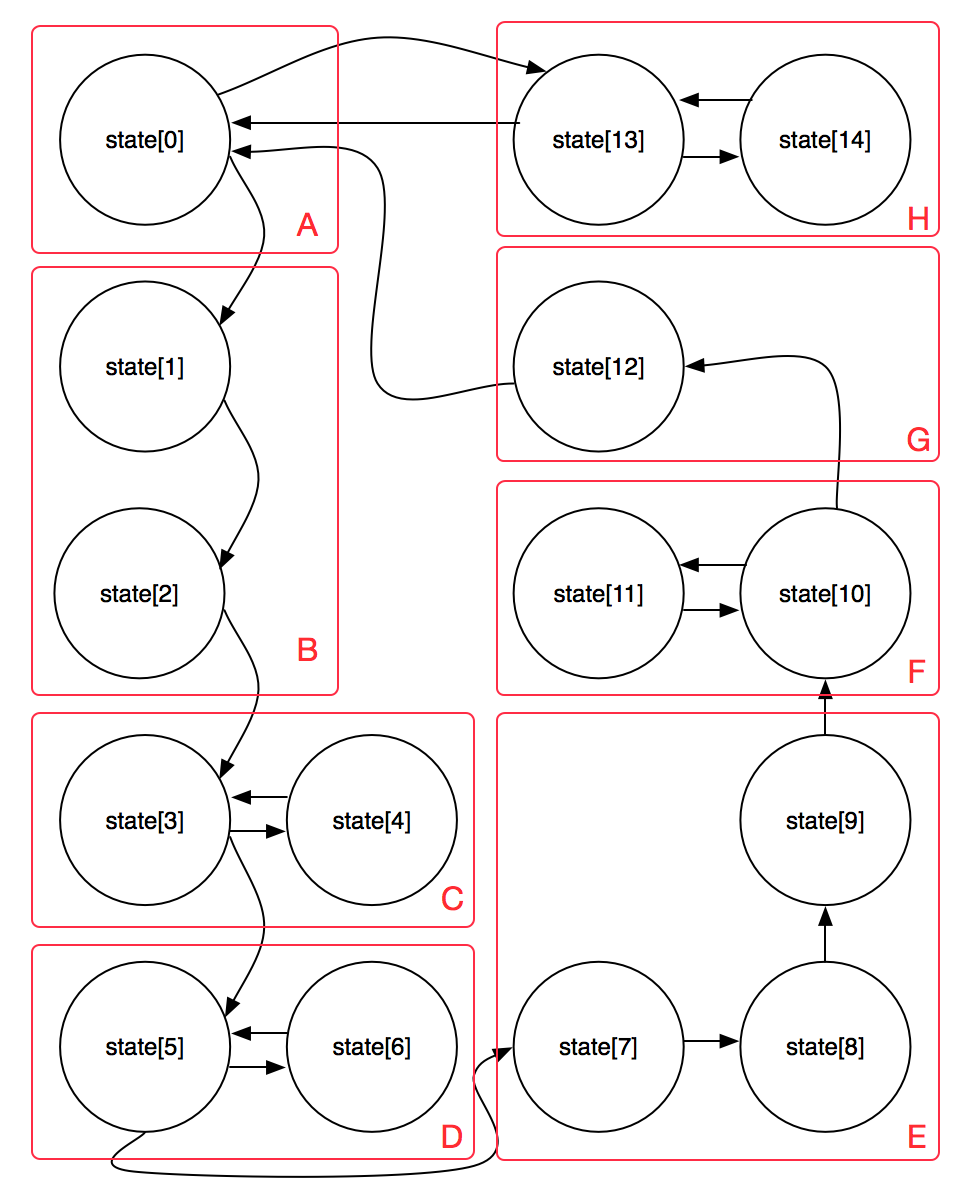
\includegraphics[width=12cm]{fsmgpu}
\caption{FSM ten behoeve van de GPU}
\label{fsmgpu}
\end{figure}




\chapter{VGA}
De VGA-controller zorgt ervoor dat een beeldscherm van de juiste signalen wordt voorzien om een beeld te kunnen opbouwen. Hierbij wordt een serieel signaal vanuit het SRAM omgezet naar een signaal dat voor een monitor is te begrijpen. Hiervoor zijn vijf signalen nodig. Drie signalen voor respectievelijk rood, groen en blauw, een voor H-Sync en een voor V-Sync. 

\begin{figure}[H]
\center
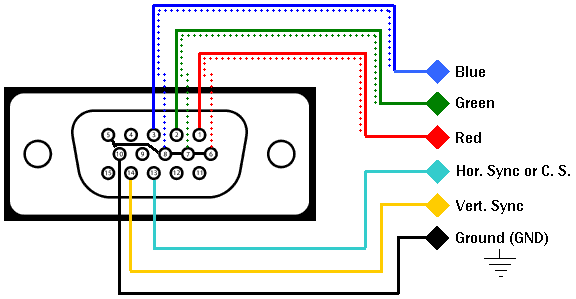
\includegraphics[width=9cm]{vga2arcade}
\caption{Layout VGA-stekker}
\label{VGA}
\end{figure}

Kortom, de VGA controller zorgt voor een H-sync, een V-Sync en dat het RGB signaal op de juiste manier aan het scherm wordt doorgegeven. 

\begin{figure}[H]
\center
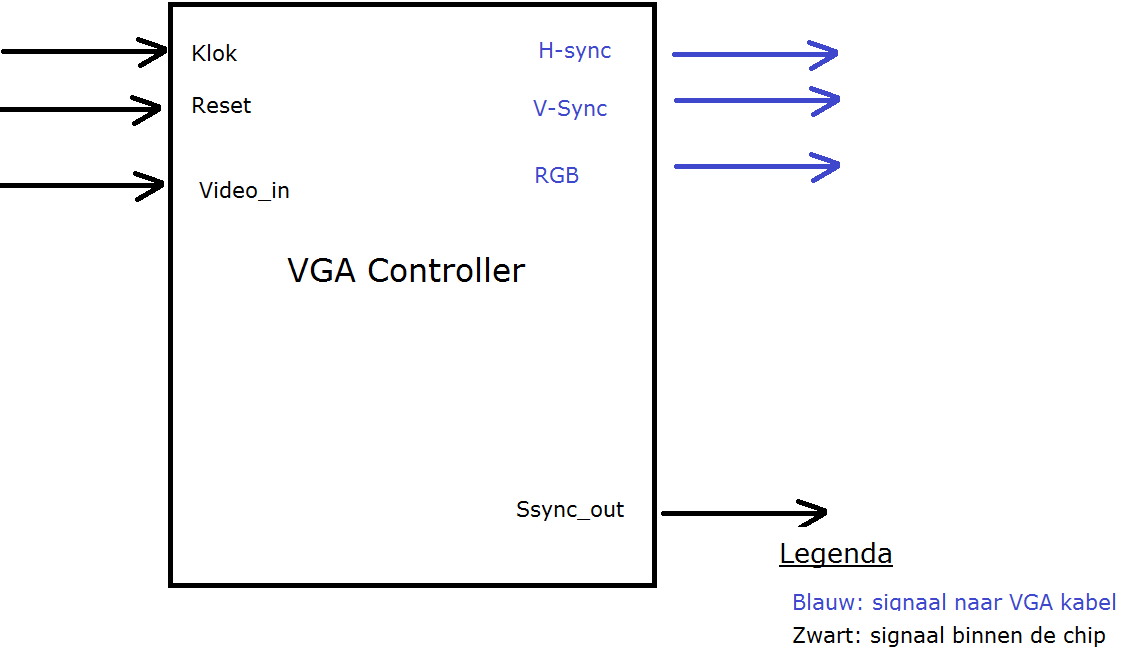
\includegraphics[width=9cm]{totaal-overzicht}
\caption{Grafische omschrijving blackbox}
\label{VGA}
\end{figure}

\section{RGB}
Op de pinnen voor rood, groen en blauw, staat een analoog signaal tussen de 0 en de 0.7 volt. Hoe hoger de spanning, hoe feller de kleur. Door middel van verschillende spanningsniveaus kan de kleur per pixel worden bepaald. Wij maken echter alleen gebruik van zwart en wit. Daarom wordt er slechts een signaal naar de alle RGB pinnen verstuurd. Hierdoor ontstaat een witte pixel. Wanneer dit niet gebeurt, is de pixel zwart. Op de FPGA wordt een digitaal signaal omgezet naar een analoog signaal tussen de 0 en 0.7 volt. Op de uiteindelijke chip zal er echter nog een schakeling nodig zijn om dit voor elkaar te krijgen. 

\section{H-Sync}
H-Sync vertelt de monitor wanneer een regel klaar. Als H-Sync laag is, betekent dit voor de monitor dat er een nieuwe regel pixels geschreven kan worden. Het is echter niet zo dat wanneer H-Sync weer hoog is, dat er gelijk pixels geschreven kunnen worden. Er zit nogal enige vertragingstijd ingebouwd. Deze tijd was bij CRT-monitoren nodig om elektronenstraal terug naar het begin te richten.

\begin{figure}[H]
\center
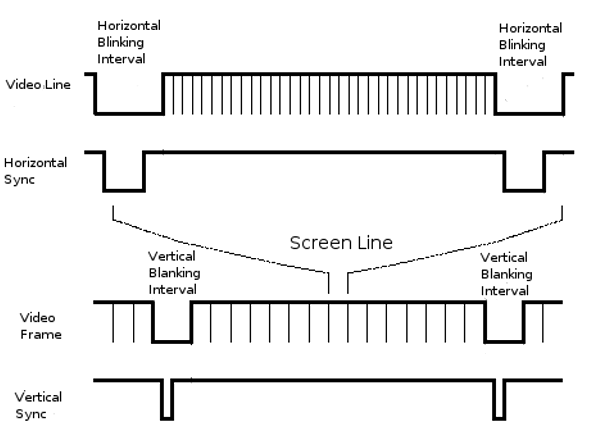
\includegraphics[width=9cm]{VGA_signal_format}
\caption{}
\label{VGA}
\end{figure}

Video Line is het RGB signaal. Zoals te zien is in figuur \ref{VGA}, zit er tijd voor en na de dip van de H-sync. Deze tijd heet de front-porch en de back-porch. 

\section{V-Sync}
V-Sync is het signaal dat aan de monitor vertelt dat een volledig scherm is volgeschreven. Als V-Sync laag wordt, begint het scherm weer links bovenin met pixels vullen. Net als bij de H-Sync is er sprake van een Front-porch en een Back-porch. Deze zijn bij de V-Sync een stuk langer dan bij de H-sync. Dit komt omdat de monitor de elektronenstraal van rechts onderin naar links bovenin moet sturen. Deze afstand is een stuk groter dan terug van rechts naar links. 

\section{Timing}
De klok van de chip is 6.177 Mhz. Op de FPGA wordt echter een klok gebruikt van 6 Mhz. Deze wordt ook aangehouden in de VHDL code. Om de counters in de VGA-controller niet te groot te maken, wordt de klok eerst gedeeld door vijf. Hierdoor is de nieuwe klok 1.2 Mhz. Wanneer er wordt gesproken van een kloksignaal, wordt er gesproken over de klok van 1.2 Mhz.

\subsection{H-Sync}
De Front-porch van de H-sync is precies één klok slag. Na de Front-porch is de H-sync vijf klokslagen laag. Daarna is de H-sync 34 klokslagen hoog. Het videosignaal naar de monitor is echter iets later pas beschikbaar. Dit komt doordat er nog een Back-porch is van twee klokslagen. 

\begin{figure}[H]
\center
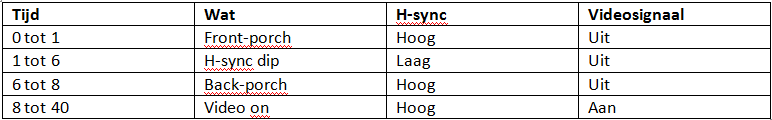
\includegraphics[width=9cm]{tabel-VGA-1}
\caption{Timing voor de H-Sync}
\label{VGA}
\end{figure}

\subsection{V-Sync}
De V-sync werkt eigenlijk op een zelfde manier als de H-Sync. Hier wordt echter niet de klok geteld, maar het aantal regels. Omdat het aantal regels een stuk minder is dan het aantal klokslagen, wordt de counter voor de V-sync (vidcounter) een stuk kleiner. Iedere keer dat het signaal voor de H-sync weer opnieuw begint, krijgt de vidcounter een signaal. Dit signaal heet nline-out. De Front-porch voor de V-Sync is 11 regels. De V-sync dip is 2 regels en de Back-porch is 31 regels. Vervolgens zijn er 480 regels beschikbaar om een videosignaal uit te zenden.

\begin{figure}[H]
\center
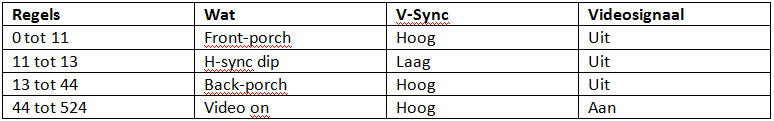
\includegraphics[width=9cm]{tabel-VGA-2}
\caption{Timing voor de V-Sync}
\label{VGA}
\end{figure}

Er wordt echter maar een keer per twintig regels een nieuw signaal op het videosignaal gezet. Hierdoor zijn er dus twintig maal zo weinig regels beschikbaar. De resolutie wordt hierdoor 32 bij 24 pixels.

\section{VHDL}
Om alle signalen op het juiste moment naar de monitor te sturen, is de VGA-controller in delen opgedeeld. 
Deler
Counter
H-sync
Vidcounter
V-sync
RGB

\begin{figure}[H]
\center
\includegraphics[width=9cm]{schema-zonder-SRAM}
\caption{Schema van de componenten}
\label{VGA}
\end{figure}

\subsection{Deler}
Dit component deelt de klok door vijf. Hierdoor is de klok 1.2 Mhz. Wanneer er over een klok gesproken wordt binnen de VGA-controller, gaat het over de klok van 1.2 Mhz.

\subsection{Counter}
Dit component telt klokslagen. Bij een resolutie van 32 bij 24 pixels, is de pixelklok gelijk aan de gedeelde klok van 1.2 Mhz. Iedere 1/1.2e6 seconde (mits von en line-on hoog zijn) komt er een nieuwe pixel op het scherm. De counter telt tot en met 40 en gaat daarna weer terug naar nul.

\subsection{H-Sync}
Dit component is een FSM. De input is de counter-vector (6 bit). De outputs zijn: Von, N-line en H-sync. Von en N-line blijven binnen de chip en H-sync wordt op de VGA uitgang gezet.

\begin{figure}[H]
\center
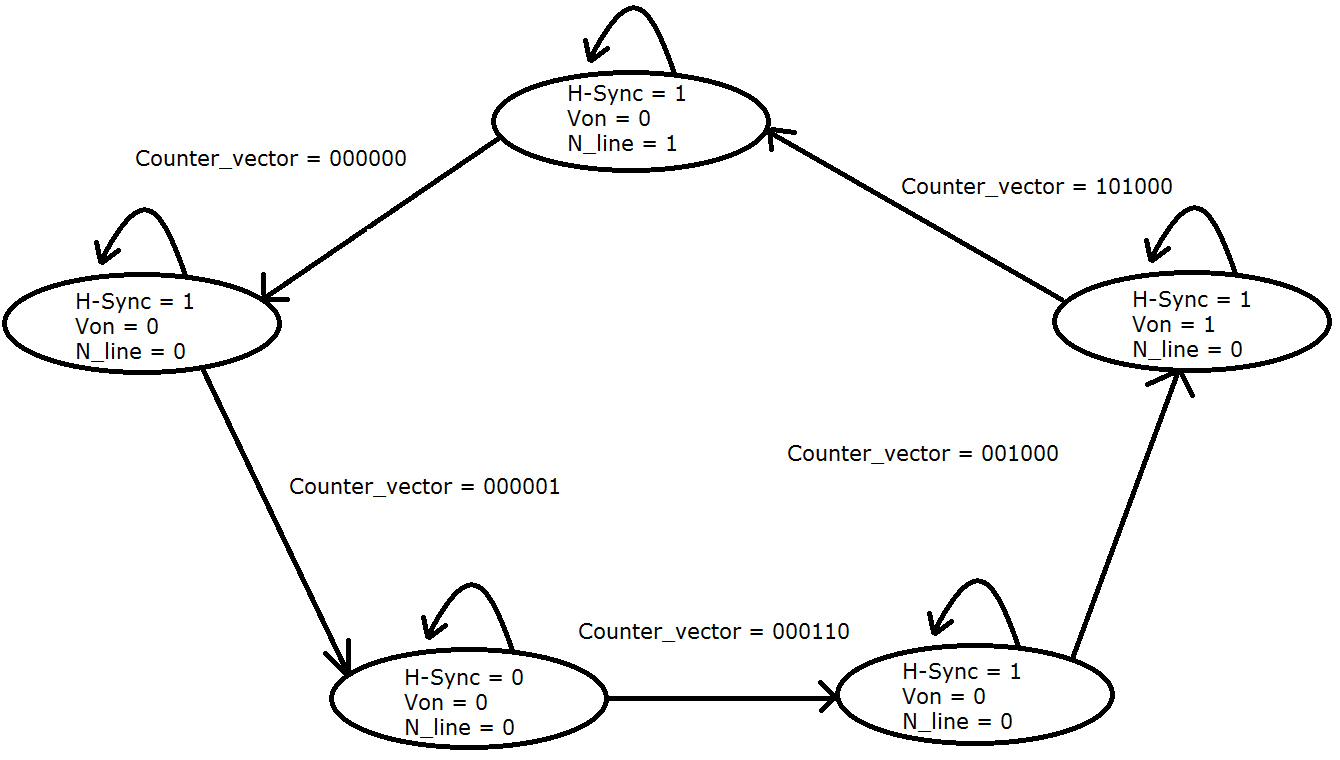
\includegraphics[width=9cm]{FSM-H-sync}
\caption{FSM H-Sync}
\label{VGA}
\end{figure}

\subsection{Vidcounter}
Dit component werkt hetzelfde als de counter. Het enige verschil is dat nu niet de klok wordt geteld, maar het signaal N-line. N-line is 1 op het moment dat er een nieuwe regel begint. De vidcounter is de counter voor de V-sync. De counter telt tot en met 524 en gaat daarna weer terug naar nul.

\subsection{V-Sync}
Dit is een FSM. De input is vid-counter-vector (10 bit). De outputs zijn V-sync, line-on en Ssync. Ssync en line-on blijven binnen de chip en V-sync wordt op de VGA uitgang gezet.

\begin{figure}[H]
\center
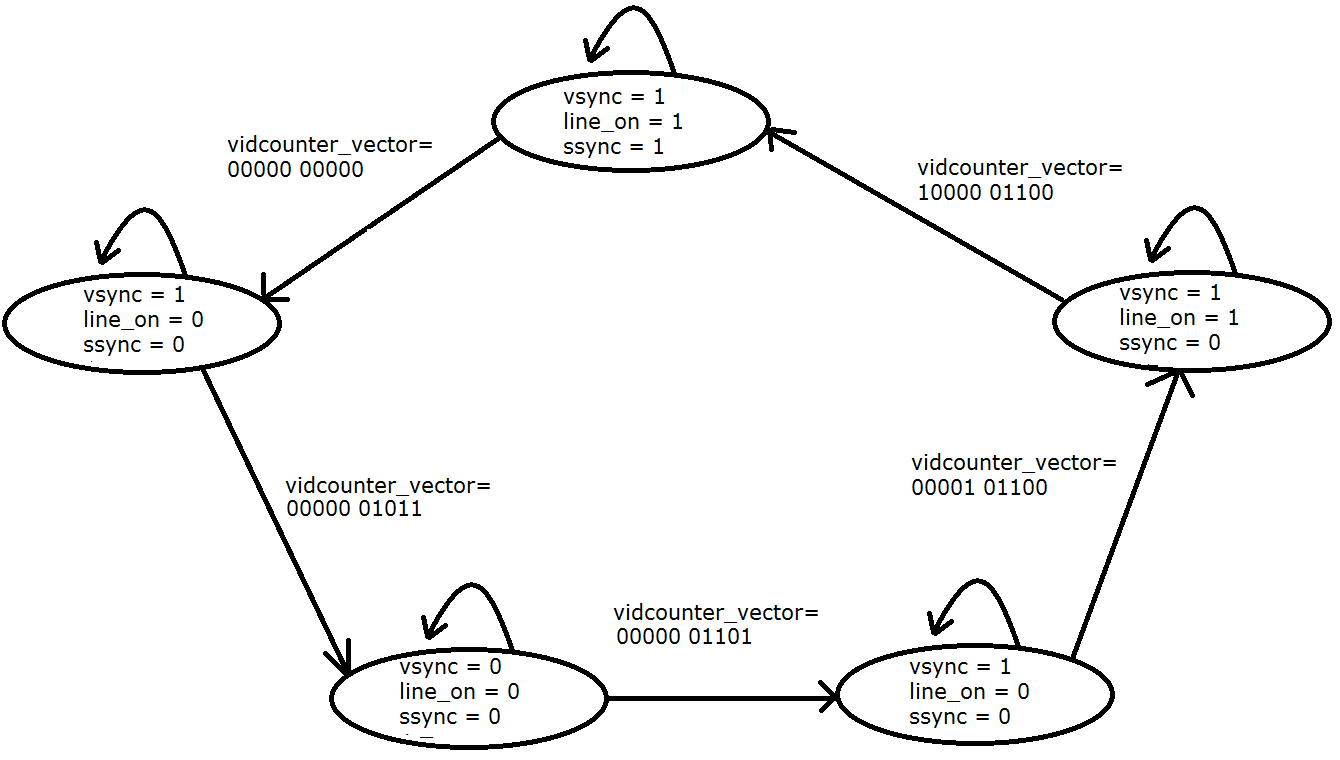
\includegraphics[width=9cm]{FSM-V-sync}
\caption{FSM V-Sync}
\label{VGA}
\end{figure}

\subsection{RGB}
Dit component zorgt ervoor dat er pixels op het scherm ingekleurd kunnen worden. Op het moment dat Von en Line-on beide 1 zijn, zit video-in aan de uitgang RGB. Dit signaal wordt de op VGA poort gezet en daarmee rechtstreeks naar het scherm gestuurd. 

\begin{figure}[H]
\center
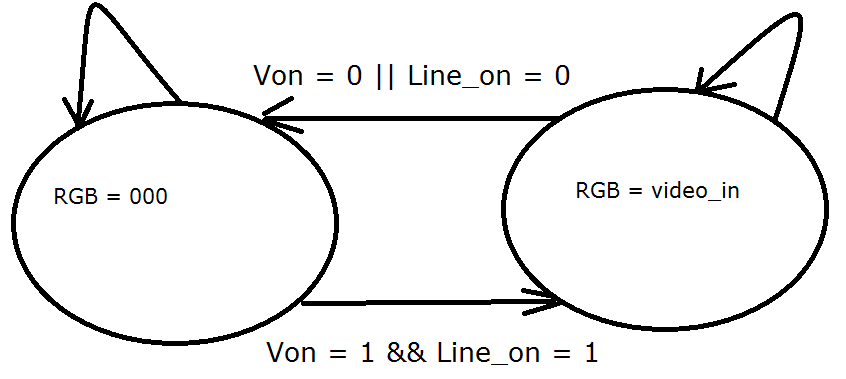
\includegraphics[width=9cm]{FSM-rgb}
\caption{FSM RGB}
\label{VGA}
\end{figure}

\section{Videosignaal}
Het videosignaal komt uit het SRAM. Om het SRAM de juiste waarden naar de VGA-controller te laten sturen, zijn er een aantal dingen nodig.
Adres
Leescommando
Sklok.
De Sklok is vrij eenvoudig. Dit is namelijk de klok waarop het SRAM bits moet gaan sturen. Aangezien er binnen de VGA controller wordt gewerkt met een klok van 1.2 Mhz, hoeft dit signaal alleen te worden doorgestuurd. Het leescommando voor het SRAM is 0000 0011. Na het leescommando, moet het adres worden gegeven. Dit adres is 0000 0000 0000 0000. Kortom, er dient een signaal van 24 bit te worden verstuurd op de klok naar het SRAM. Na dit signaal, gaat het SRAM direct waarden gegeven. Het is dus belangrijk dat op de laatste regel de 24 bits worden verstuurd zodat er op de eerste regel direct kan worden uitgelezen. Hiervoor is het signaal Ssync. Dit komt uit de V-sync. 

\begin{figure}[H]
\center
\includegraphics[width=9cm]{schema-met-SRAM}
\caption{Schema van de componenten}
\label{VGA}
\end{figure}

\subsection{S-synccounter}
Deze counter begint met tellen als Ssync hoog is. Vervolgens telt de counter tot 40. Daarna begint hij weer opnieuw.

\subsection{S-Sync}
Net als de H-Sync en V-Sync is dit een FSM met ongeveer dezelfde werking. 

\begin{figure}[H]
\center
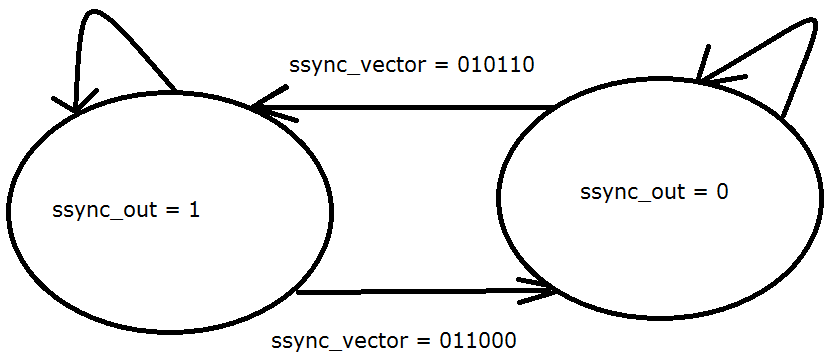
\includegraphics[width=9cm]{FSM-Ssync}
\caption{FSM Ssync}
\label{VGA}
\end{figure}

\section{Conclusie}
Om alle signalen op het juiste moment naar de monitor te sturen, is de VGA-controller in zes delen opgedeeld. Daarnaast zijn er nog twee componenten nodig om het SSRAM aan te sturen. Hierdoor komt het totaal op acht componenten uit. 
Deler
Counter
H-sync
Vidcounter
V-sync
RGB
Ssync-counter
Ssync

\section{Resultaten}
Op de foto is een testscherm te zien. Hierbij zijn enkele pixels te zien in verschillende kleuren.

\begin{figure}[H]
\center
\includegraphics[width=9cm]{resultaat}
\caption{Testscherm vanaf de FPGA}
\label{VGA}
\end{figure}

\chapter{SPI}
Serial Peripheral Interface in het kort ook SPI genoemd is een de facto-standaard die ooit door Motorola bedacht is voor het communiceren met randapparatuur, zoals embedded systems, sensors en memory cards. Omdat SPI niet een officiële standaard is er geen specificatie om aan te houden bij het ontwerpen, om toch een refentie te hebben is er gebruikt gemaakt van \cite{motorola} waarin het ontwerp van een SPI module wordt omschreven. Bij SPI heb je de master en de slave deze communiceren met elkaar via twee seriële datalijnen daarnaast is er nog een kloklijn die aangeeft wanneer er data overgedragen wordt. De kloklijn wordt aangestuurd door de master, dit houdt in dat de slave niet kan pauzeren en altijd data aan de master aan moet bieden. De standaard definieert enkel hoe de data van de master naar de slave en vice versa over wordt gedragen, niet hoe de data verwerkt wordt, dit heeft als gevolgd dat randapparatuur zelf nog moet definiëren hoe de communicatie verloopt.

\section{Functionele beschrijving}
De SPI module begint met zenden/ontvangen zodra het send signaal hoog is en stopt zodra er acht bits zijn verzonden/ontvangen, daarna kunnen de ontvangen bits uitgelezen worden en nieuwe bits in worden geladen om te verzenden. Het overbrengen van het shift register dat in de master zit naar de slave en vice versa deze shift registers zijn in een kring op elkaar aangesloten, waarbij altijd de meest significante bit wordt verzonden. Voor de communicatie met de slave wordt een slave klok signaal gegenereerd, de data overdracht is gesynchroniseerd ten opzicht van dit signaal. Data wordt gesampled op de opgaande klokflank en de data wordt geshift op de neergaande klokflank, een verduidelijking van hoe deze timing precies werkt is te zien in figuur \ref{spi-timing-diagram}

\begin{figure}[H]
\center
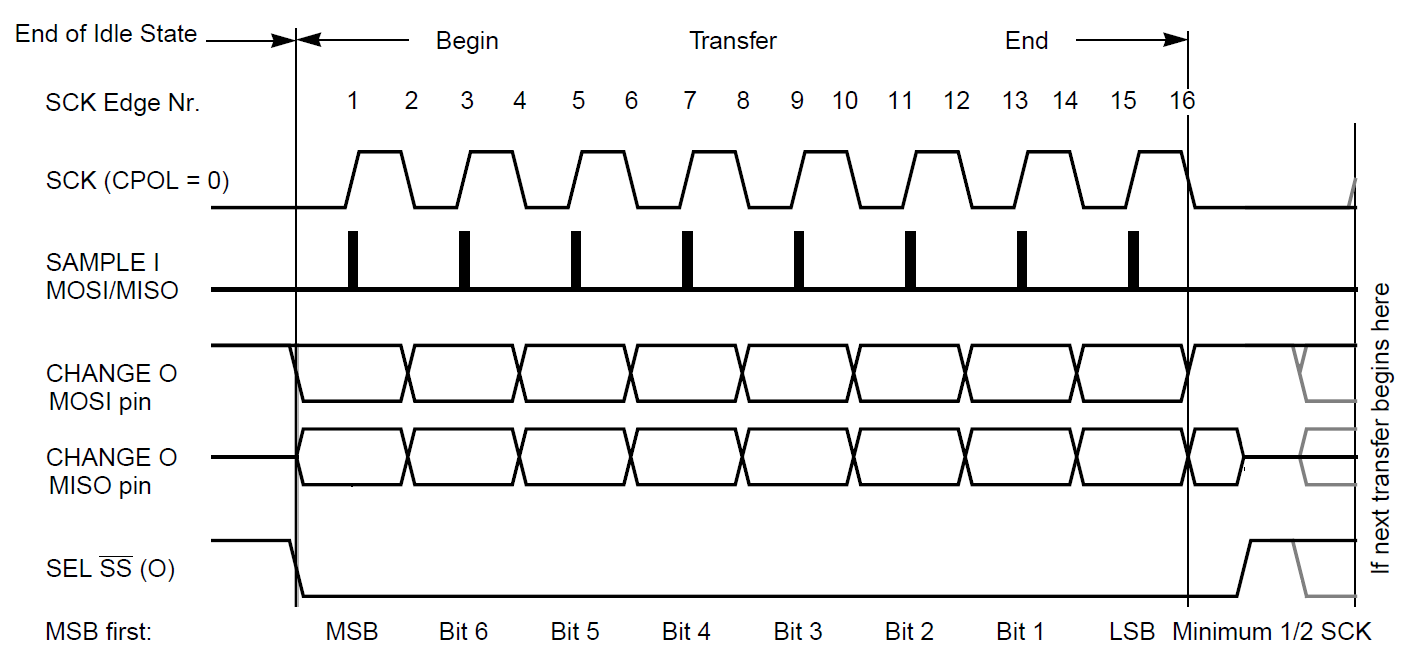
\includegraphics[width=15cm]{./spi_timing_diagram}
\caption{Diagram van SPI timing}
\label{spi-timing-diagram}
\end{figure}

\section{Inputs en outputs}
Hieronder een beschrijving van alle in- en outputs van de SPI module zoals te zien in figuur \ref{spi-diagram}.
\begin{itemize}
\item Clock: het kloksignaal waarop de SPI draait, het slave clock signaal zal dezelfde frequency hebben als dit kloksignaal
\item Reset: de hoofd reset van de SPI
\item Send: de input die aangeeft wanneer er begonnen moet worden met zenden/ontvangen
\item Write\_enable: als deze hoog is zal write\_in(8) in het shift register geladen worden
\item Write\_in(8): de bits die naar het shift register worden geschreven als write\_enable hoog is
\item Read\_out(8): de waarde die in het shift register staat
\item Slave clock: het slave kloksignaal die de communicatie met de slave aanstuurt
\item MOSI: de datalijn van de master naar de slave
\item MISO: de datalijn van de slave naar de master
\end{itemize}

\begin{figure}[H]
\center
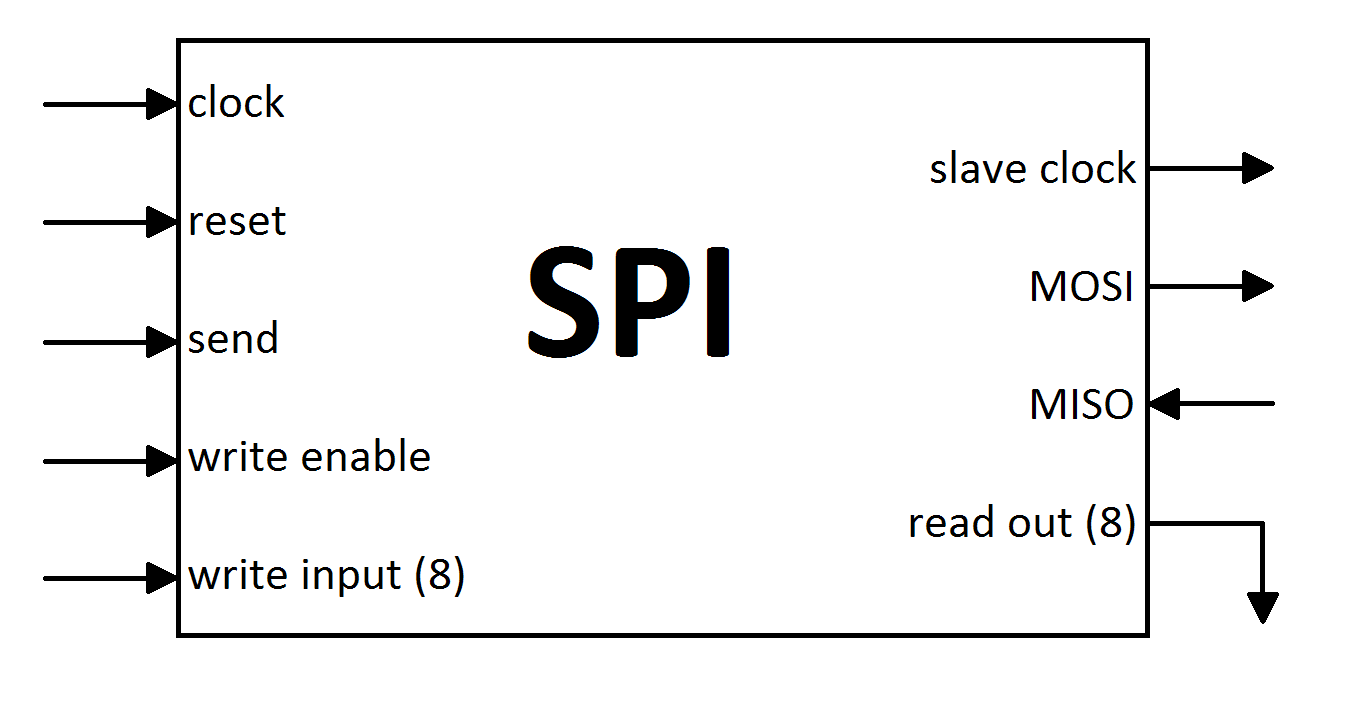
\includegraphics[width=7cm]{./spi_diagram}
\caption{Diagram van SPI circuit}
\label{spi-diagram}
\end{figure}

\section{Implementatie}
Voor de implementatie van de SPI is er voor gekozen om het in drie subsystemen op te delen:
\begin{itemize}
\item Counter: een simpele teller die de opgaande klokslagen van het slave clock signaal telt. 
\item Shift register: een shift register van acht bits die shift op de neergaande klokflank als het enable signaal hoog is en nieuwe waardes inlaad als de write enable hoog is. Het blokschema van het shift register is te zien in figuur \ref{shift-register-diagram}.
\item Control: een statemachine die er voor zorgt dat de SPI stopt met shiften na 8 klokslagen van de slave klok, zodat er tijd is om het register uit te lezen of nieuwe waarden in te laden. Het blokschema van Control is te zien in figuur \ref{control-diagram}.
\end{itemize}

Deze drie subsystemen zijn aan elkaar verbonden volgens het schema in figuur \ref{spi-system-diagram}.

\begin{figure}[H]
\centering
\begin{minipage}{.5\textwidth}
  \centering
  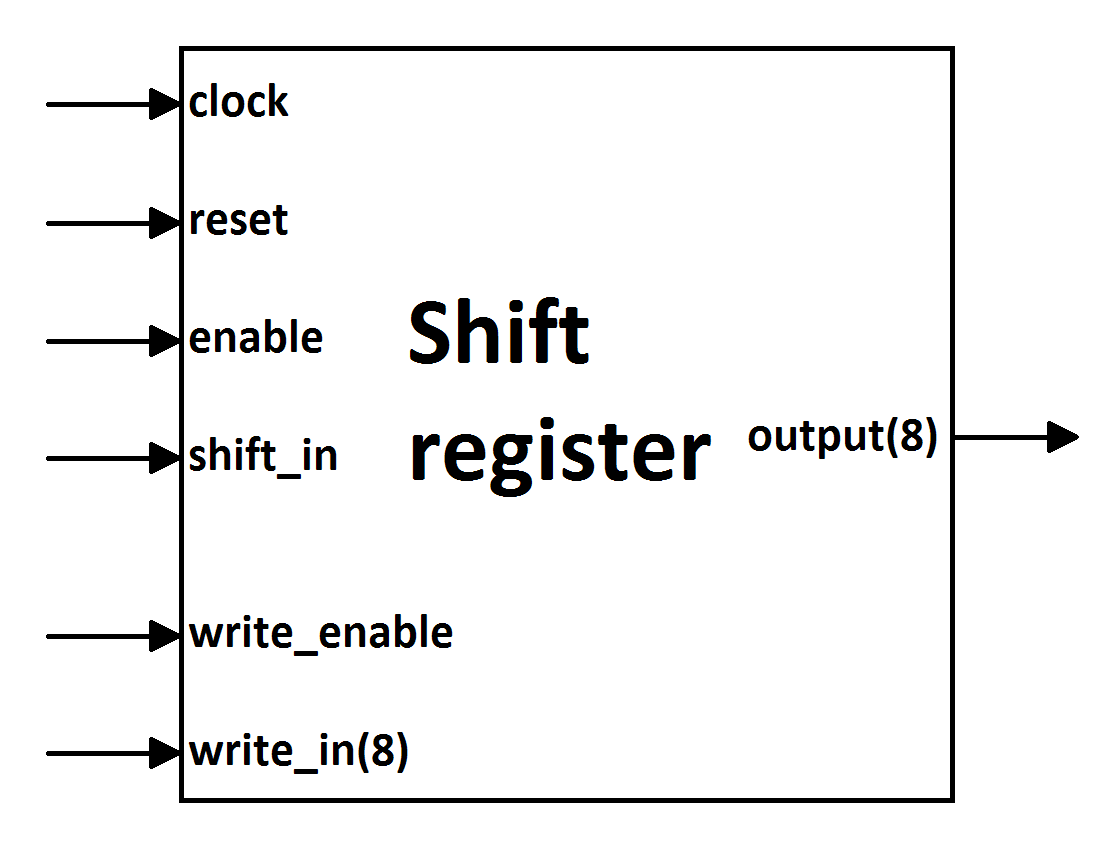
\includegraphics[width=5.4cm]{./shift_register_diagram}
  \captionof{figure}{Diagram van Shift regiser}
  \label{shift-register-diagram}
\end{minipage}%
\begin{minipage}{.5\textwidth}
  \centering
  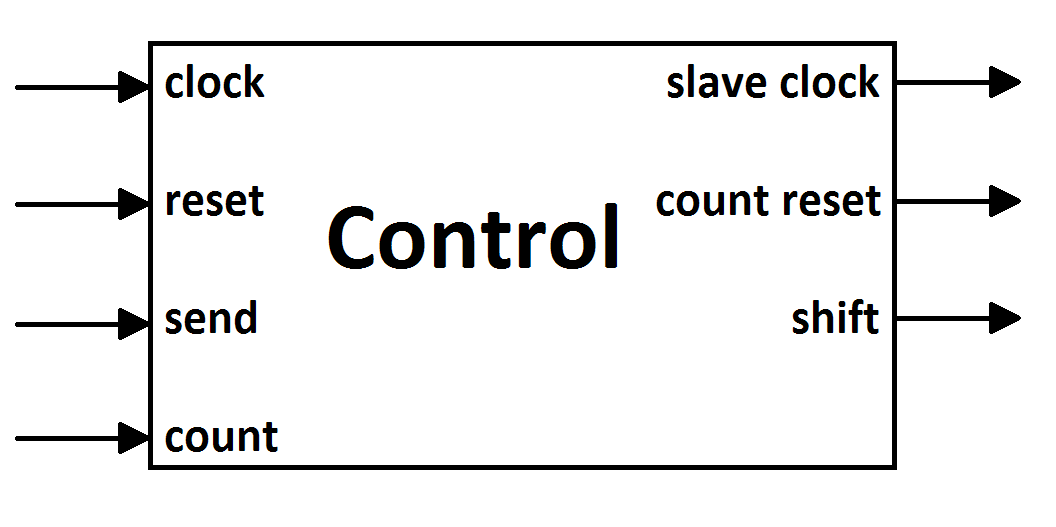
\includegraphics[width=7.8cm]{./control_diagram}
  \captionof{figure}{Diagram van Control} 
  \label{control-diagram}
\end{minipage}
\end{figure}

\begin{figure}[H]
\center
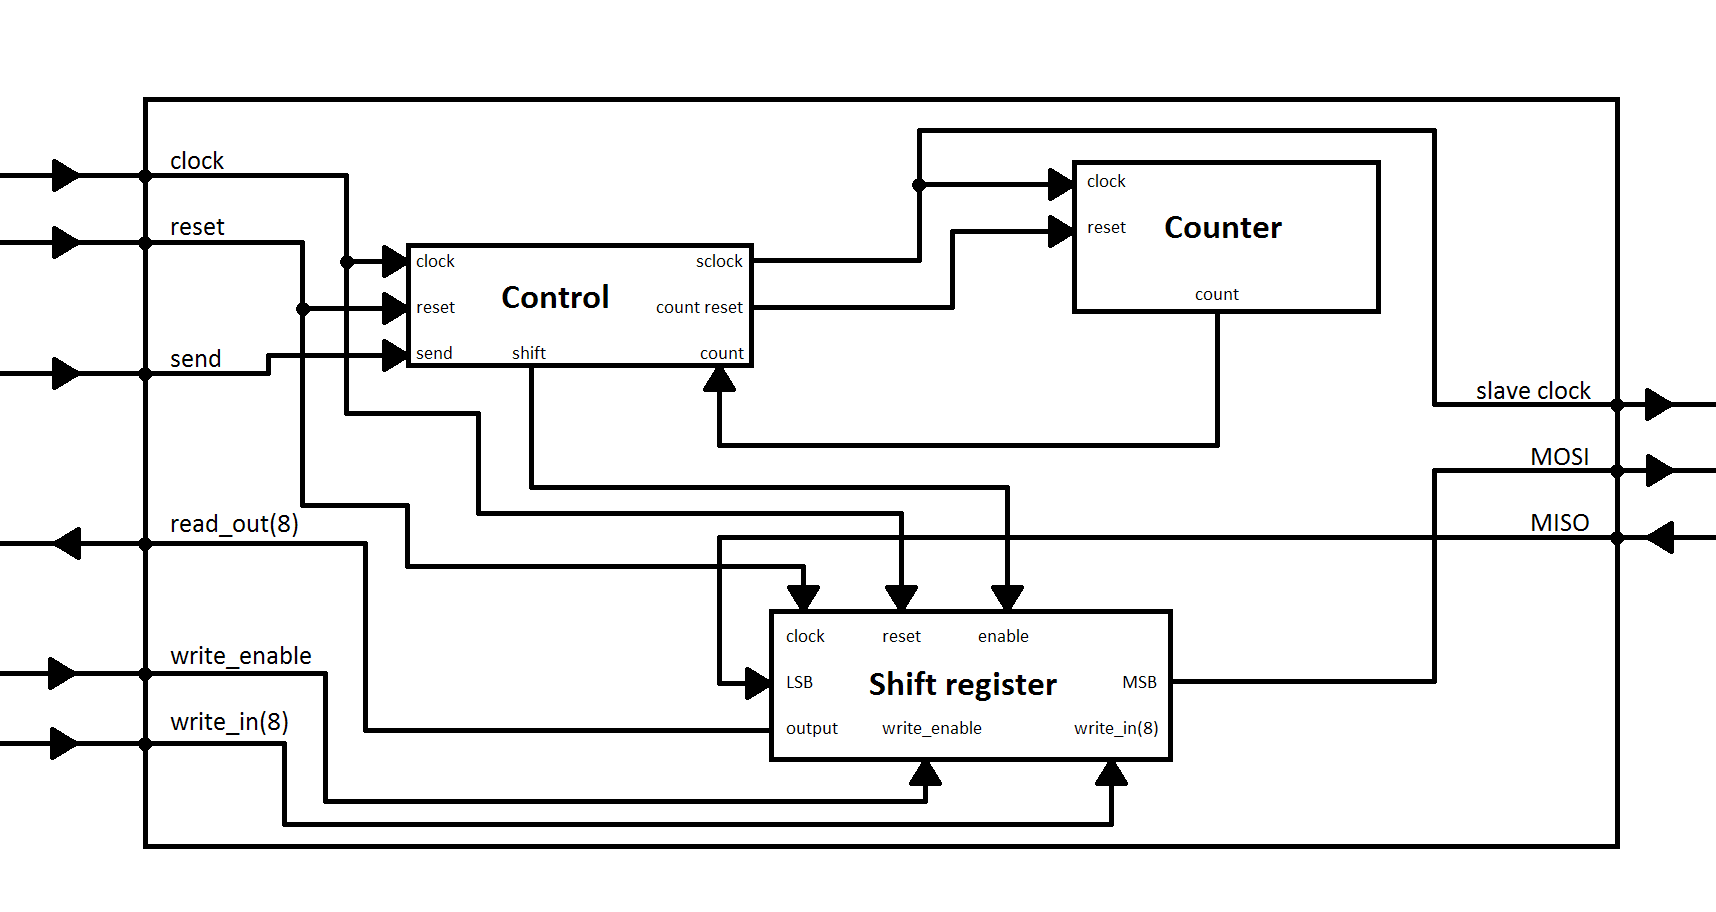
\includegraphics[width=11.4cm]{./spi_system_diagram}
\caption{Diagram van de verbinding van de componenten}
\label{spi-system-diagram}
\end{figure}

\newpage

\chapter{SD-kaart}
Voor het opslaan van de instructies voor de CPU is gekozen voor een SD-kaart. Voor het uitlezen van een SD-kaart zijn er drie verschillende modes, twee hiervan zijn echter gebaseerd op een zelf ontworpen systeem van SanDisk. De derde mode is echter gebaseerd op SPI waarvan al een module is die al ontworpen is, daarom is hier ook voor gekozen. 
\section{SD communicatie}
Aangezien SPI niets zegt over hoe de communicatie verloopt of wat de betekenis van de overgebrachte data is, definieert SanDisk in de SD specificatie een aantal commando’s die naar de SD-kaart gestuurd kunnen worden. De specificatie die gebruikt is is uit 2003, dit is omdat dit de enige volledige specificatie is die te vinden was. Dit is omdat je een licentie bij SanDisk moet hebben om toegang te hebben tot de meest recente en volledige specificaties.
\section{SD commando's \& responses}
De communicatie met de SD-kaart verloopt als volgt: er wordt een commando naar de SD-kaart verstuurt, de SD-kaart geeft antwoordt of het een correct commando is en of het commando verwerkt kan worden, daarna komt eventueel nog, bij het lezen, data van de SD-kaart of, bij het schrijven, data naar de SD-kaart. Zodra alles is afgehandeld kan er een nieuw commando gestuurd worden. Hoe dit precies verloopt is te zien in figuur \ref{sd-cmd-diagram} hierin is data versturen naar de SD-kaart weggelaten omdat hier geen gebruik van wordt gemaakt.

\begin{figure}[H]
\center
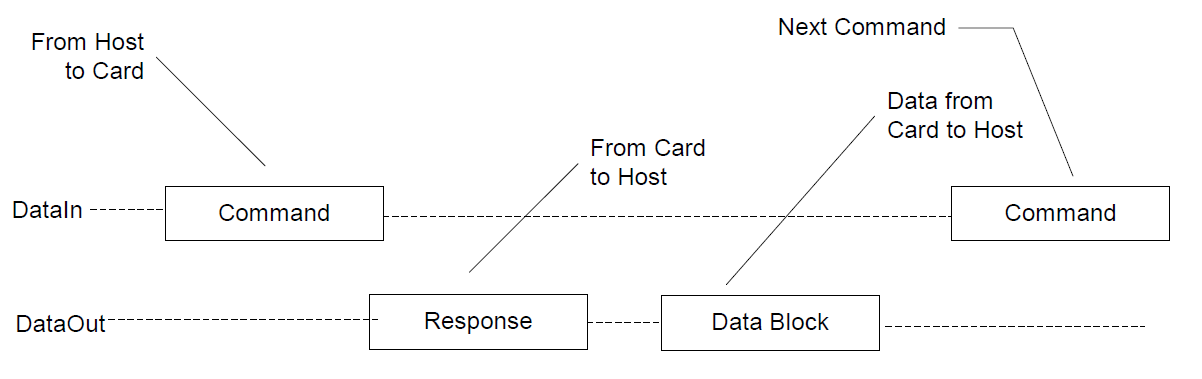
\includegraphics[width=14cm]{./sd_cmd_diagram}
\caption{Commando communicatie van SD-kaart}
\label{sd-cmd-diagram}
\end{figure}

\section{Functionele omschrijving}
De SD module is zo ontworpen dat deze een adres binnen krijgt van de program counter van de CPU deze uitleest vanaf de SD-kaart en deze vervolgens aanbiedt aan de CPU. Zolang de SD module nog bezig is met het uitlezen van het adres zal het busy signaal hoog zijn.

\begin{figure}[H]
\center
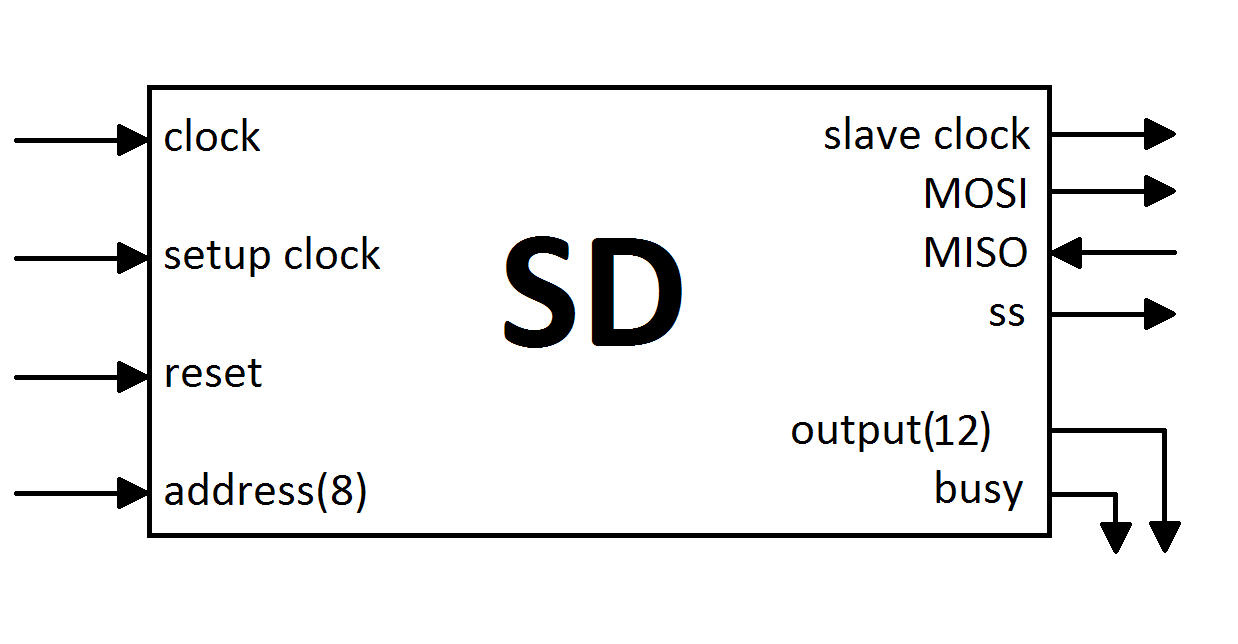
\includegraphics[width=7cm]{./sd_diagram}
\caption{Diagram van SD-kaart}
\label{sd-diagram}
\end{figure}

\newpage

\section{Inputs en outputs}
Hieronder een beschrijving van alle in- en outputs van de SD module zoals te zien in figuur \ref{sd-diagram}.

\begin{itemize}
\item Clock: het kloksignaal waar de SD module op draait, dit is ook het kloksignaal waar de SPI na initialisatie op zal draaien
\item Setup clock: het kloksignaal dat tijdens de initialisatie gebruikt zal worden, deze moet tussen de 100 en 400 kHz liggen
\item Reset: het algemene reset signaal 
\item Address: het adres dat van de SD-kaart zal worden afgelezen
\item Output(12): dit zal de waarde zijn die op het adres staat zodra deze is uitgelezen
\item Busy: dit signaal geeft aan of de SD module bezig is
\item Slave clock: het slave kloksignaal dat de SD-kaart aanstuurd
\item MOSI: de datalijn van de SD module naar de SD-kaart
\item MISO: de datalijn van de SD-kaart naar de SD module
\item SS: het slave select signaal, dit signaal wordt gebruikt om de SD-kaart in SPI mode te krijgen en om aan te geven dat de SD-kaart geselecteerd is.
\end{itemize}

\chapter{Conclusie en Aanbevelingen}
\section{Conclusie}
Het EPO-3 project van de bachelor opleiding Electrical Engineering begon in tegen stelling tot voorgaande projecten vrij soepel. Als groep waren we het snel met elkaar eens, het zou een spelcomputer worden met een ultrasone besturing. Gaande weg liepen we tegen steeds meer dingen aan. \\

Ons plan, het bouwen en ontwerpen van een spelcomputer, is achteraf niet haalbaar geweest. Het is ons niet gelukt alle individuele onderdelen op tijd werkend te krijgen. Beide opslag units zorgden hier voor het grootste probleem. De SD-kaart uitlezing leek telkens te werken, maar stopte er telkens tijdens het testen mee. Omdat op de SD-kaart de spellen opgeslagen worden en dit dus de basis vormt voor de spelcomputer. Bleek dit niet realiseerbaar meer en zijn we overgestapt op een ander plan. Met de componenten die werkend zijn gekregen is een simpele rekenmachine ontworpen. 

\section{Aanbevelingen}
Achter af is het natuurlijk simpeler gezegd als gedaan, maar het is bij dit EPO-3 project belangrijk een duidelijk doel te stellen. Er moet daarbij vooral gelet worden op de haalbaarheid van het ontwerp. Het is met deze vrijheid in keuze dan ook gevaarlijk om te veel te willen realiseren. Dit heeft bij onze project groep voor veel stress gezorgd, wat zeker niet ideaal is aan het einde van een periode. 

\chapter{Discussie}
\section{Reflectie op het eindontwerp}
Zoals eerder in het verslag al aangegeven is het ons niet gelukt om een werkende spelcomputer te realiseren. Met de werkende onderdelen zijn we vervolgens verder gegaan en hebben een simpele rekenmachine ontworpen. De problemen die we tijdens het proces tegen kwamen zaten vooral in de communicatie tussen de FPGA en de externe componenten. Het lukte ons niet om de SD-kaart uitlezing werkend te krijgen. Deze leek telkens te werken, maar was onmogelijk stabiel te krijgen. Dit zelfde probleem ondervonden we met beide SRAM geheugens. Deze onderdelen leken het hele project haalbaar, pas in de laatste week kwamen de problemen naar voren. Dit had tot gevolg dat het onmogelijk geworden was iets sterkers te produceren dan dat ons nu gelukt is. 

\section{Reflectie op het groepsproces}
EPO-3 groep A5 begon dit project sterk en georganiseerd, dit was grotendeels te danken aan onze voorzitter Erné Bronkhorst. Beslissingen konden gezamenlijk en snel worden genomen, dit gaf ons een goede voorsprong. Ook de taakverdeling en planning leek erg soepel te lopen. Gaande weg het project werd steeds meer duidelijk dat niet alle onderdelen evenveel tijd kosten, dit had tot gevolg dat er achteraf in moest worden gesprongen in onderdelen en dat koste erg veel tijd. De besturing was daar een goed voorbeeld van, deze kon eigenlijk vrij snel gerealiseerd worden. Hierdoor kwamen er twee mensen zonder taak te zitten, gelukkig kon dit vrij snel worden opgelost. Er moest nog een plan van aanpak worden geschreven en een toplevel beschrijving ontworpen. In de laatste fase van het project heeft de taakverdeling ervoor gezorgd dat we dit toch nog met een goed resultaat konden beëindigen. 

 \begin{thebibliography}{1}

  \bibitem{motorola} SPI Block Guide, http://www.ee.nmt.edu/~teare/ee308l/datasheets/S12SPIV3.pdf, benaderd in oktober en november. 2014.

  \end{thebibliography}

\appendix

\chapter{Plan van aanpak}
\section{Achtergronden}
Door onze aanmelding bij de studie Electrical Engineering aan de TU-Delft hebben wij van deze organisatie opdracht gekregen om een eigen chip te ontwerpen, verder is alles geheel voor eigen keuze. De opdracht zal door de opdrachtgevers gekozen naam 'Ontwerp een chip' benoemd worden. Dit project is aangenomen door alle leden van de projectgroep A5, tevens zal dit project worden begeleid door Dr. R. Ishihara. Dr. R. Ishihara zal hiernaast fungeren als onze tutor. Deze opdracht zal binnen de Technische Universiteit Delft worden verwerkt. Dit project speelt in op de in college naar voren gekomen onderdelen, waaronder 'Programmeren in C' en 'Digitale systemen'. Het dient als doel onze kennis te verdiepen en te verbreden in de elektrotechniek. De uiteindelijke stakeholders zijn behalve de opdrachtgevers, daardoor ook de projectnemers. Deze opdracht is een onderdeel en vereiste voor het behalen van de Bachelor opleiding 'Electrical Engineering'.

\section{Projectresultaat}
Tijdens het EPO-3 project 'Ontwerp een chip' dient een chip ontworpen te worden, dit kan bijvoorbeeld het implementeren van een spelletje of een Infrarood-Besturing op een chip zijn. Deze opdracht mag door de projectgroep gekozen worden. Bij het ontwerp van de chip dient gebruik gemaakt te worden van Sea-of-gates technologie.

\subsection{Doelstellingen van het project}
Allereerst is het doel van het project, het succesvol uitvoeren van de opdracht gekregen van de opdrachtgever. Belangrijk hierbij is het ontwerpen aan de hand van globale productspecificaties met randvoorwaarden. Daarnaast, zeker niet onbelangrijk, zijn de vaardigheden die universiteit ons mee wilt geven. Deze vaardigheden komen gaandeweg het project steeds meer naar voren.  Hierbij speelt projectmatig werken in een groep een grote rol. Ook worden de projectnemers middels dit project getraind in vergaderen, overleggen en plannen. Als laatst worden verschillende technische vaardigheden in de praktijk getraind waaronder programmeren, simuleren en het bouwen van verschillende schakelingen. Er moet tijdens dit EPO-3 project strikt worden gelet op het combineren en testen van de verschillende ontwerpen, hierbij kan worden gebruik gemaakt van moderne computerhulpmiddelen. De projectleden zullen gaande weg dit project hierin gesteund en getest worden.  

\subsection{Eindresultaat}
Als eindresultaat zal er een chip moeten worden ontworpen, daarnaast moet er een verslag worden geschreven.
De chip moet aan een aantal eisen voldoen, namelijk:
\begin{enumerate}
\item Op de chip moet een spelcomputer gebouwd worden, deze spelcomputer dient spelletjes van een SD-kaart te kunnen weergeven op een beeldscherm.
\item Ultrasone sensoren moeten de besturing vormen voor de spelcomputer.
\item Er moet minimaal een spel ontworpen worden (Pong). Mocht er tijd over zijn dan kunnen er meer spelletjes ontworpen worden.
\item Het beeld dient te worden weergegeven met VGA op een beeldscherm.
\end{enumerate}
Ook het verslag moet aan een aantal eisen voldoen:
\begin{enumerate}
\item Het verslag bestaat uit twee delen, het technische verslag en het procesverslag.
\item Het technisch verslag documenteert de ontwerpkeuzes en de prestaties van de chip.
\item De weekverslagen/notulen vormen een basis voor het procesverslag.
\item Het verslag dient te worden geschreven volgens het format van de projecthandleiding.
\end{enumerate}

\section{Projectactiviteiten}
Het project kan worden opgedeeld in het uitvoeren van de volgende taken:
\begin{enumerate}
\item Opstellen plan van aanpak
\begin{itemize}
\item verzamelen en bestuderen informatie
\item maken van concept plan van aanpak
\item bespreken plan van aanpak met opdrachtgever
\end{itemize}
\item Ontwerpen en bouwen besturing
\item Ontwerpen microprocessor
\item Ontwerpen en bouwen geheugenelement (SD)
\item Ontwerpen VGA + SRAM module
\item Schrijven Pong (spelletje)
\end{enumerate}

\section{Projectgrenzen}
In dit project is veel vrijheid gegeven door de opdrachtgever. Dat neemt niet weg dat er aan een aantal eisen moet worden voldaan, voornamelijk de beperkingen die de chip met zich mee brengt. Deze eisen staan beschreven in de projecthandleiding, en zijn hieronder even kort samengevat.
\begin{enumerate}
\item Het ontwerp dient klaar te zijn binnen het 2e kwartaal.
\item De schakeling dient te werken op een klokfrequentie van 6.144 MHz.
\item Elke projectgroep heeft 0.4 $cm^2$ ruimte op de chip, dit komt overeen met 40.000 transistor paren.
\item Per groep zijn er 32 aansluitpinnen beschikbaar.
\item Voor de FSM's mogen alleen die van het type Moore gebruikt worden, daarnaast moet er altijd een reset aanwezig zijn.
\item Het streven is om zo weinig mogelijk componenten extern te gebruiken.
\end{enumerate}

\subsection{Tussenresultaten}
De tussenresultaten van dit project worden uitgebreid beschreven in het gehele tussentijdse ontwerprapport en dus niet verder behandeld in het plan van aanpak.

\subsection{Kwaliteitsbewaking}
\textbf{Eindproduct}\\
Het eindproduct van het derde project van de bachelor Electrical Engineering moet een goed werkende chip zijn die aan enkelen eisen voldoet, deze eisen zijn door de projectgroep zelf opgesteld:\
\begin{itemize}
\item Op de chip moet een spelcomputer gebouwd worden, deze spelcomputer dient spelletjes van een SD-kaart te kunnen weergeven op een beeldscherm.
\item Ultrasone sensoren moeten de besturing vormen voor de spelcomputer.
\item Er moet minimaal een spel ontworpen worden (Pong). Mocht er tijd over zijn dan kunnen er meer spelletjes ontworpen worden.
\item Het beeld dient te worden weergegeven met VGA op een beeldscherm.
\end{itemize}
\textbf{Controles}\\
Tussendoor zullen er een aantal controles worden uitgevoerd om de kwaliteit te blijven bewaken, namelijk:
\begin{itemize}
\item Is het haalbaar om spelletjes extern te laden?
\item Werkt de uitlees module van de SD-kaart?
\item Is de ultrasone sensor besturing bruikbaar voor het eindresultaat?
\item Lukt het om met de VGA een beeld op een scherm te printen? 
\end{itemize}
Deze punten zullen voornamelijk worden gecontroleerd door de groep zelf. Hierbij is er duidelijk een leider aangewezen die het overzicht behoud en zo de voortgang van het project controleert. Daarnaast vindt er nog een docentcontrole gaande weg tijdens het project plaats om de kwaliteit te bewaken, deze kan worden gedaan door de hoofddocent of door een van zijn assistenten.

\section{Projectorganisatie}
\textbf{Organisatie}\\
De projectgroep EPO-3 A5 bestaat uit acht leden. Om het overzicht te behouden is er een voorzitter benoemd. De voorzitter is Ern\'e Bronkhorst.
Verder bestaat de projectgroep uit:
\begin{itemize}
\item Marc Zwalua (Notulist)
\item Niels de Winter
\item Wietse Bouwmeester
\item Bauke Meekes
\item Job Tijhuis
\item Hans Okkerman
\item Jordy van der Horst
\end{itemize}
\textbf{Onderlinge afspraken:}
\begin{itemize}
\item Om de voortgang te bewaken zal er wekelijks een evaluatie plaatsvinden waarin dit wordt bekeken. Hierin wordt zo nodig de planning voor de komende weken bijgesteld.
\item Als groepsleden horen wij altijd op tijd en verplicht aanwezig te zijn bij elke geplande bijeenkomst. Als dit onverwachts niet mogelijk is, zal hier zo snel mogelijk melding van gemaakt moeten worden. 
\item Als er onderlinge geschillen zijn, dan worden deze besproken met de hoofddocent. Dit zorgt ervoor dat de voortgang niet in gevaar komt.
\item Alle groepsleden moeten garant staan voor een gelijke bijdrage aan het project.
\end{itemize}
\textbf{Verantwoording}\\
Er zal constant tijdens de project middagen mondeling gerapporteerd worden over de voortgang van het project. Schriftelijk wordt er halverwege de periode een mid-term rapport geschreven, hierin wordt de voortgang opgenomen. De verantwoording zal bij Dr. R. Ishihara worden gedaan. 

\subsection{Planning}
Een duidelijk schema van onze planning is toegevoegd als bijlage.

\subsection{Risicoanalyse}
Hier volgt een overzicht van de eventuele risico's die we tijdens EPO-3 tegen zouden kunnen komen. Door middel van deze analyse worden deze risico's zoveel mogelijk vermeden.
\textbf{Externe risico's:}
\begin{itemize}
\item Onduidelijke informatie voorziening.
\item Onvoldoende feedback vanuit de docenten
\end{itemize}
\textbf{Interne risico's:}
\begin{itemize}
\item Verliezen van meetresultaten.
\item Botsing tussen de groepsleden.
\item Het eventueel ontbreken van kennis of inzet onder de groepsleden.
\item Het project niet af kunnen ronden door een tekort aan tijd.
\end{itemize}
Een aantal interne risico's kunnen worden vermeden door het aanstellen van de voorzitter, deze zal de voortgang bewaken en alle resultaten netjes beheren. Voor de externe risico's zal er vooral zelf moeten worden gezocht naar oplossingen in combinatie met de docenten.

\newpage
\section{Bijlage}
\begin{figure}[h]
  \centering
  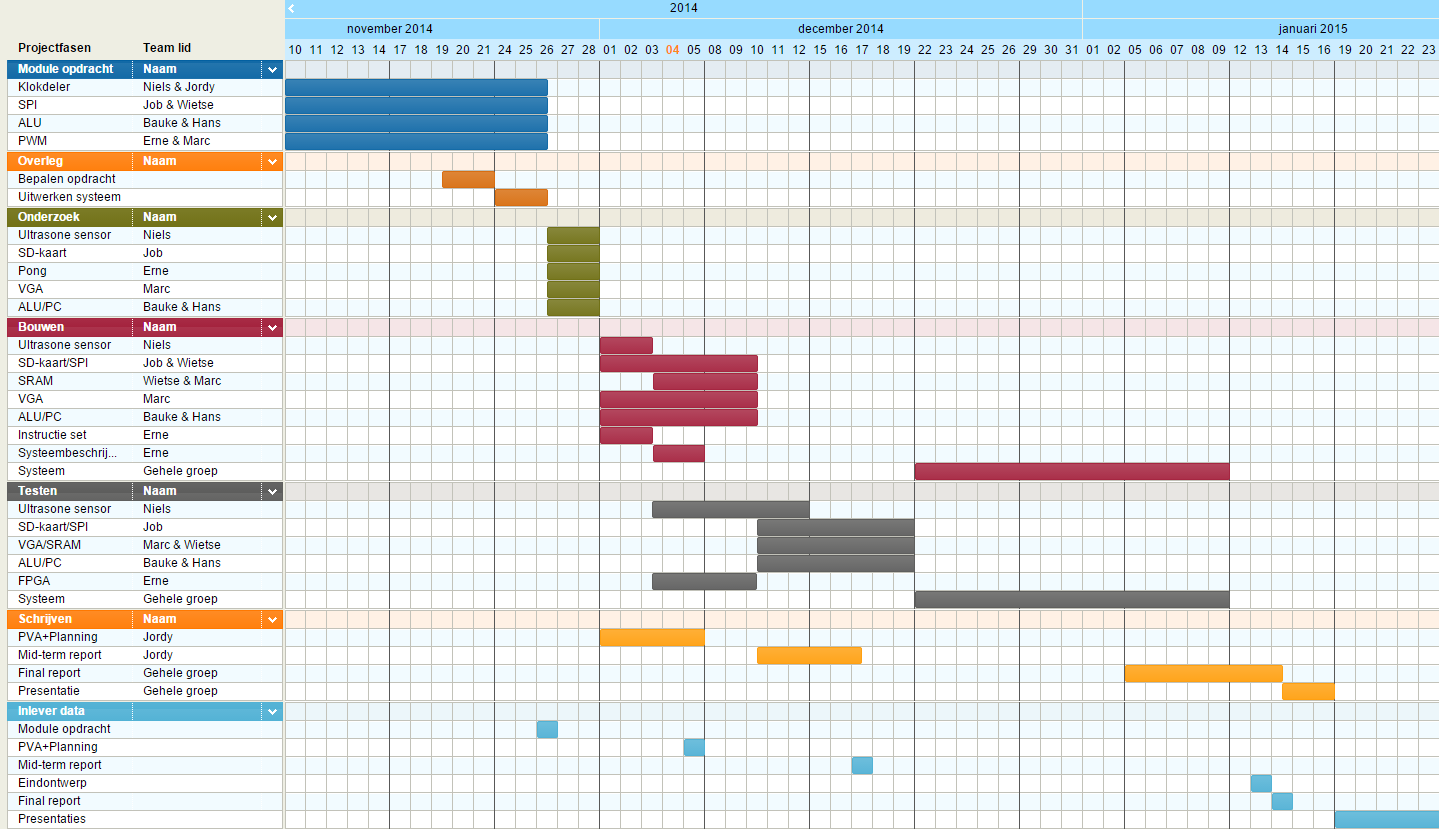
\includegraphics[width=15.5cm,  angle=-90]{Planning}
    \caption{Planning A5} 
\end{figure}


\chapter{Bijlage - VHDL bestanden}
\section{Blackbox}
\label{Blackbox entity}
\lstinputlisting[language=VHDL]{VHDL/blackbox.vhd} 
\label{Blackbox behaviour}
\lstinputlisting[language=VHDL]{VHDL/blackbox-behaviour.vhd}
\label{Stream entity}
\lstinputlisting[language=VHDL]{VHDL/stream.vhd}
\label{Stream behaviour}
\lstinputlisting[language=VHDL]{VHDL/stream-behaviour.vhd}

\section{ROM}
\label{ROM}
\lstinputlisting[language=VHDL]{VHDL/rom.vhd}

\section{CPU}
\label{}
\lstinputlisting[language=VHDL]{VHDL/alu.vhd}
\label{}
\lstinputlisting[language=VHDL]{VHDL/cpu.vhd}
\label{}
\lstinputlisting[language=VHDL]{VHDL/cpu_EXTR.vhd}
\label{}
\lstinputlisting[language=VHDL]{VHDL/cpu_tb.vhd}
\lstinputlisting[language=VHDL]{VHDL/pc_counter.vhd}
\lstinputlisting[language=VHDL]{VHDL/decoder.vhd}
\lstinputlisting[language=VHDL]{VHDL/gates.vhd}

\section{Buffers}
\lstinputlisting[language=VHDL]{VHDL/buf_2.vhd}
\lstinputlisting[language=VHDL]{VHDL/buf_3.vhd}
\lstinputlisting[language=VHDL]{VHDL/buf_4.vhd}
\lstinputlisting[language=VHDL]{VHDL/buf_5.vhd}
\lstinputlisting[language=VHDL]{VHDL/buf_6.vhd}
\lstinputlisting[language=VHDL]{VHDL/buf_7.vhd}
\lstinputlisting[language=VHDL]{VHDL/buf_8.vhd}
\lstinputlisting[language=VHDL]{VHDL/buf_9.vhd}
\lstinputlisting[language=VHDL]{VHDL/buf_10.vhd}
\lstinputlisting[language=VHDL]{VHDL/buf_A.vhd}
\lstinputlisting[language=VHDL]{VHDL/buf_arg.vhd}
\lstinputlisting[language=VHDL]{VHDL/buf_i.vhd}
\lstinputlisting[language=VHDL]{VHDL/instr_buf.vhd}

\section{Registers}
\lstinputlisting[language=VHDL]{VHDL/reg_2.vhd}
\lstinputlisting[language=VHDL]{VHDL/reg_3.vhd}
\lstinputlisting[language=VHDL]{VHDL/reg_4.vhd}
\lstinputlisting[language=VHDL]{VHDL/reg_5.vhd}
\lstinputlisting[language=VHDL]{VHDL/reg_5.vhd}
\lstinputlisting[language=VHDL]{VHDL/reg_6.vhd}
\lstinputlisting[language=VHDL]{VHDL/reg_7.vhd}
\lstinputlisting[language=VHDL]{VHDL/reg_8.vhd.vhd}\lstinputlisting[language=VHDL]{VHDL/reg_9.vhd}
\lstinputlisting[language=VHDL]{VHDL/reg_10.vhd}
\lstinputlisting[language=VHDL]{VHDL/reg_a.vhd}
\lstinputlisting[language=VHDL]{VHDL/reg_cluster.vhd}
\lstinputlisting[language=VHDL]{VHDL/reg_o.vhd}
\lstinputlisting[language=VHDL]{VHDL/shift_reg.vhd}

\section{Gate}
\lstinputlisting[language=VHDL]{VHDL/gate.vhd}

\section{GPU}
\lstinputlisting[language=VHDL]{VHDL/gpu.vhd}
\section{Calculator}
\lstinputlisting[language=VHDL]{VHDL/calculator.vhd}
\lstinputlisting[language=VHDL]{VHDL/tb.vhd}


\end{document}

